\documentclass[oneside,a4paper,11pt,openrany]{book}

%openright

\usepackage{ThesisStyle}
% \usepackage{apacite}	% - For the bibliography
\usepackage[square,numbers]{natbib}
\usepackage{comment}
\usepackage[usenames]{color}
\usepackage[spanish, es-tabla]{babel}
\usepackage{pdfpages}
\usepackage[utf8]{inputenc}
\usepackage{listings}
\usepackage{soul}
\usepackage{soulutf8}

\setboolean{@twoside}{true}	% - Setting twoside boolean to true (does not change margin)


\title{Ecosistema para el Descubrimiento de Conocimiento en Lenguaje Natural} % - Thesis name

\begin{document}

%%TC:ignore

	%	<Cover>	%
	%\include{./Chapters/Cover/Cover}
	\begin{titlepage}

\center % Center everything on the page


%----------------------------------------------------------------------------------------
%	LOGO SECTION
%----------------------------------------------------------------------------------------

\includegraphics[scale=.60]{./Images//Chapters/Cover/UA.jpg}\\[.5cm] % Include a department/university logo - this will require the graphicx package



%----------------------------------------------------------------------------------------
%	HEADING SECTIONS
%----------------------------------------------------------------------------------------
{\Large Departamento de Lenguajes y Sistemas Inform{\'a}ticos}\\[0.25cm] % Department
{\Large Escuela Polit{\'e}cnica Superior}\\[2.0cm] % University

%----------------------------------------------------------------------------------------
%	TITLE SECTION
%----------------------------------------------------------------------------------------

%\HRule \\[0.4cm]
{ \huge \bfseries Ecosistema para el}\\[0.3cm]
{ \huge \bfseries Descubrimiento de Conocimiento}\\[0.3cm]
{ \huge \bfseries en Lenguaje Natural}\\[1.5cm] % Thesis title
%\HRule \\[1.5cm]

%----------------------------------------------------------------------------------------
%	AUTHOR SECTION
%----------------------------------------------------------------------------------------

{ \LARGE Alejandro Piad Morffis}\\[1.5cm]


%----------------------------------------------------------------------------------------
%	PROGRAM SECTION
%----------------------------------------------------------------------------------------

{ \it Tesis presentada para aspirar al grado de }\\[.25cm]
{ DOCTOR POR LA UNIVERSIDAD DE ALICANTE }\\[.25cm]
% { MENCI{\'O}N DE DOCTOR INTERNACIONAL }\\[.25cm]
{ DOCTORADO EN INFORM{\'A}TICA }\\[0.5cm]


%----------------------------------------------------------------------------------------
%	SUPERVISION SECTION
%----------------------------------------------------------------------------------------

{ \it Dirigida por }\\[.25cm]
{ Dr. Yoan Gutiérrez Vázquez \\ Dr. Yudivián Almeida Cruz \\ Dr. Rafael Muñoz Guillena }\\[1.5cm]


%----------------------------------------------------------------------------------------
%	FUNDING SECTION
%----------------------------------------------------------------------------------------

{ Esta tesis ha sido co-dirigida y financiada por\\la Universidad de Alicante y la Universidad de La Habana. }


%----------------------------------------------------------------------------------------

\vfill % Fill the rest of the page with whitespace

\end{titlepage}

	\blankpage
	{
\center

\Large{\bf TESIS DOCTORAL EN FORMA DE COMPENDIO DE PUBLICACIONES} 
\BlankLine

Ecosistema para el Descubrimiento de Conocimiento en Lenguaje Natural
\BlankLine
}

El presente documento contiene una síntesis del trabajo realizado por Alejandro Piad Morffis, bajo la dirección de Dr. Yoan Gutierrez Vazquez, Dr. Rafael Muñoz Guillena y Dr. Yudivián Almeida Cruz, para optar por el grado de Doctor en Informática. Se presenta en la Universidad de Alicante y se estructura según
la normativa establecida para la presentación de tesis doctorales en forma de compendio de publicaciones: una primera parte con una síntesis, una segunda parte que reproduce las publicaciones científicas realizadas y una tercera parte con las conclusiones.

	\blankpage

	%	<Dedication>	%
	\thispagestyle{empty}

\vspace*{\fill}

\begin{flushright}
\textit{A mi familia y amigos, por hacerme quien soy.}

\textit{A Sue, por enseñarme a querer más.}

\textit{A papá, por creer.}
\end{flushright}

\vspace*{\fill}
	%	- Dedication

	%\frontmatter
	\pagestyle{fancyUnnumberedSectionsStyle}	% - Fixing style for the regular chapters
	\chapter*{Agradecimientos}
\markboth{Agradecimientos}{}
\phantomsection
\pagenumbering{roman}

Cuando empecé la aventura que me traje al día de hoy, allá por el año 2008, yo tenía grandes expectativas pero ningún plan concreto.
Sabía que quería estudiar en la Universidad de La Habana, y que quería hacer algo con computadoras, pero nada más.
Mi padre se sentó conmigo, él al timón, yo en el asiento del acompañante, como siempre hacíamos por esa época, esperando a que mi hermana, quien entonces estudiaba violín, terminara sus clases.

Papá me preguntó cuáles eran mis aspiraciones ahora que comenzaba la Universidad.
Él siempre recordaba la Universidad como la época de su vida donde más grande se hizo su mundo, y creo que por eso quería que la mía fuera una experiencia excepcional.
Yo le dije simplemente que quería ser el mejor. El mejor de mi clase, el mejor de toda la carrera, vaya, el mejor del mundo incluso.
Y en vez de decirme cuan ridículas eran esas expectativas, me dijo ``pues hagamos un plan para lograr eso''.

Y así lo hicimos, planeamos ahí en media hora los pasos que supuestamente me iban a llevar a cumplir esas ridículas metas. Pasos que tenían que ver con dedicar no se cuántas horas a estudiar, con hacerme alumno ayudante lo antes posible, con trabajar en proyectos adicionales.
Hoy sé que no había ninguna garantía de que esos pasos me llevaran a ser el mejor del mundo, pero al menos me trajeron hasta aquí.
Y así aprendí que los sueños no están para cumplirse, están para empujarte a llegar más lejos, mucho más lejos de lo que tu pudieras imaginar, aunque muchas veces en direcciones totalmente diferentes de las que soñaste.

Este sueño lo he compartido con muchísimas personas, tantas que me es imposible agradecerles a todos por las huellas que han dejado en mi vida. Trataré de mencionar a algunos de los imprescindibles, pero pido disculpas de antemano por todos aquellos que seguro me faltarán.

En primer lugar, tengo que agradecer infinitamente a mi padre. Agradecerle por muchas cosas simples y mundanas, como enseñarme a montar bicicleta, a nadar, a disfrutar de los libros, a conducir, a comer saludable, a querer a los demás por sus defectos y no a pesar de ellos, y a soñar en grande.
Pero lo más importante que me dió mi padre no fueron ni habilidades específicas ni su filosofía de vida.
Papá siempre creyó que yo podía lograr lo que me propusiera, incluso cuando eso no coincidiera con lo que él veía más importante o valioso, incluso aunque que mis planes y expectativas me llevaran lejos de las suyas.
Y no es cierto, uno no puede lograr todo lo que se propone, claro que no.
Su propia vida estuvo llena de metas fallidas y expectativas frustradas, como la de todos.
Pero si uno no cree que puede, no tiene sentido ni siquiera intentarlo.
Y por eso el superpoder de mi padre era creer, creer que todo era posible, que solo dependía de uno mismo, y que no había obstáculo suficientemente grande.

Si bien mi padre me dio gran parte del combustible que quemé para hacer lo que he hecho, nunca lo hubiera logrado sin mi madre.
Cuando las cosas se ponían de verdad complicadas, cuando parecía que no había más solución que rendirse, mi madre siempre encontraba una salida, una forma de reinventarse para seguir adelante.
Lo hizo cuando yo era un niño y no alcanzaba la comida para los tres, lo hizo de nuevo cuando nació mi hermana, lo volvió a hacer años después cuando todo lo que tenían construido tambaleó, y después de aquel octubre de 2019 cuando la vida de todos nosotros dio un vuelco repentino y definitivo.
De mi madre aprendí muchas cosas, pero quizás la más importante es esa: que uno tiene el poder de reinventarse tantas veces como sea necesario, por uno mismo, y por los que uno quiere.
Y que nadie más que tu mismo puede realmente derrotarte.

Mi hermana ha sido la tercera constante en mi vida, o al menos la mayor parte de ella.
En muchas cosas somos muy parecidos, en otras, diametralmente opuestos.
Pero hay una cosa en especial que compartimos, una admiración mutua desde nuestro punto de vista por el otro, que nos hace estar cerca aunque haya distancia física.
Siendo yo el mayor, siempre he sentido que mi hermana es mi fan número uno.
Lo que ella no supone, porque casi nunca lo he dicho, es que yo también su fan número uno, y que a pesar de los años de supuesta ventaja que le llevo, son muchas las enseñanzas que he sacado de verla crecer, convertirse en una persona capaz de cometer sus propios errores, bajo sus propias condiciones, siendo una fuente de energía vital para muchos a su alrededor, pero sin perder su propia identidad en el proceso.
Y junto a Alenia, tengo que agradecer a Andy por acompañarla, por complementarla, y por traer a nuestra familia su júbilo, sus ganas de vivir, de reír, de cantar.
Ellos dos me han enseñado el valor de perseguir tus sueños, contra viento y marea, a pesar de todas las opiniones que puedas tener en tu contra.

Mi familia no es muy grande, y no siempre han podido estar todos los que hubiesen querido. Pero de cada uno he aprendido algo, y a cada uno le dedico también un pedacito de estas páginas.
A mi abuela Sofía, que estuvo ahí desde mis primeros días de escuela, y que sigue ahí a pesar de los pesares.
A mi abuelo Roberto, que fue un ejemplo de honradez, de trabajo duro, y de entrega por sus seres queridos, y quien desgraciadamente no pudo ver a sus nietos crecer tanto como hubierse querido, pero estoy seguro estaría orgulloso.
A mi abuelo Pepín, que a pesar de lo poco que pudo compartir conmigo, guardo recuerdos hermosos. A mis tíos y primos por ambas partes de la familia, que han estado en momentos buenos, y algunos en otros momentos no tan buenos.
A mi tío Frank en especial por el cariño incondicional, y a mi primo Francito, como siempre le llamaré, por tantas horas que compartimos de niños, y las que seguro nos quedan por compartir.

Quiero agradecer también a mi segunda familia, la que no me tocaba, pero me acogió como si fuera un hijo más.
A mis suegros, Estela y Armando, que me enseñaron a ver la vida de forma un poco diferente; sus enseñanzas sí que me han marcado, mucho más de lo imaginan, y mucha culpa tienen de la persona que soy hoy.
A Wendy, que ha sido una hermana más, por su forma de sentir y querer que no conoce fronteras ni limitaciones; y a Daniel, por su amistad, y por darme algunas de las horas de conversación más interesantes que he tenido.
A mis abuelos postizos, Mimi, Gregorio, Ondina, y Armando, por su cariño immerecido; a Tony y Betty, Alain y Yahima, por hacerme parte de su familia.
Y a todos los demás, tíos, primos, y abuelos, por acogerme como uno más en todos los momentos.

Amigos tengo muchísismos, algunos desde siempre, otros desde hace poco, y todos han dejado una huella en mi.
En especial quiero agradecir a mis amigos del alma, con los que viví tres años compartiéndolo todo, desde el agua y la comida hasta las aspiraciones, los sueños, y las ganas de vivir.
A Silvio, Charly, Ian Pedro, Pepito, y Luis Alberto, no tengo forma de agradecerles por tantos años de estar ahí, en las buenas y en las malas, aunque estemos desperdigados por todos los continentes.
A mis amigos y compañeros de la UH, con los que he aprendido no solo habilidades y conocimientos, sino formas nuevas de pensar y de ver la vida.
A mis amigos de Alicante, de España, y del resto del mundo, que me han abierto los horizontes y me han dado nuevas esperanzas y expectativas.
De todos ellos me llevo un trocito, y espero que todos tengan en cambio algo de mí.
Y quiero agradecer también a los más chiquitos, que fueron mis estudiantes y ahora se han convertido en compañeros, a Jonpi, Roci, Daniel, Hian, Sadán, Estevanell, y todos los que vienen en camino.
Ellos son mi mayor fuente de orgullo, y por cada cosa que hayan podido aprender de mi, hay algo que he aprendido también de ellos.

Desde mis primeras letras hasta el día de hoy, todo lo que pueda haber logrado lo debo en gran medida a mis profesores, que me enseñaron a leer, a sumar, a derivar, a programar, a escribir artículos, a hablar en público, a dirigir un proyecto.
Son demasiados para nombrarlos a todos, pero sepan que los recuerdo.
En especial, quiero agradecer a Marrero, por inspirarme su amor por la ciencia, y enseñarme la belleza que hay en entender el universo.
A Lupi, por prestarme atención en aquel primer año, y empujarme siempre a saber más.
A Bolu, por enseñarme a pensar como un científico, y animarme a seguir esta vida.
A Luciano y Katrib, por inspirarme con su energía inagotable y demostrarme que no hay cansancio que valga si uno ama su trabajo.
Por supuesto, a mis tutores de Alicante, Yoan, Rafa y Andrés, por confiar en mi, y guiarme por este camino con infinita paciencia.
Y muy especialmente, a Yudy, por ser maestro y amigo, por enseñarme que podía aspirar a más aunque el resto del mundo no estuviera de acuerdo, y por estar siempre dispuesto a compartir este sueño.

Finalmente, quiero agradecer a mi esposa, mi mejor amiga, y mi inseparable compañera de equipo, Suilan.
Ella me ha enseñado demasiadas cosas para resumirlas aquí, pero la lección más importante que he aprendido es que, en última instancia, nadie más que tú puede decirte que algo es imposible.
Suilan expandió mi universo rompiendo límites que yo ni me daba cuenta que existían, y se atrevió a caminar por ese universo conmigo, compartiendo miles de horas de frustración, pero también innumerables alegrías.
Ella es mi mayor crítico, mi más valioso consejero, y el más importante miembro en todos mis equipos.
Nada de lo que pueda decir aquí sería suficiente para resaltar la importancia que ha tenido su presencia en mi vida, como una gigante roja cuya fuerza gravitacional cambia todo a años luz de distancia.
De no haberla conocido, no tengo idea de dónde estaría, pero seguro seríamos ambos muy diferentes a cómo somos.
Y por si fuera poco, me ha dado la alegría mayor de saber que pronto seremos padres, y tendremos así una nueva aventura, seguramente más difícil como todas las anteriores, pero que también compartiremos juntos.

Cuando empecé este viaje hace más de 13 años, nunca imaginé donde estaría hoy.
Imaginé muchas cosas, algunas que pasaron, y muchas otras que no pasaron.
Por el camino he aprendido tantas cosas, cosas sobre el mundo, y cosas sobre mí, que no estoy seguro de pueda decir que aquella persona que empezó con aquel plan en aquella tarde 2008 sea la misma que escribe estas letras.
Muchas puertas se me abrieron, gracias a muchas personas que no he alcanzado a mencionar, así como otras puertas se cerraron.
He camino por aquellas que consideré mejor, y aunque estoy seguro que muchas veces dejé ir oportunidades que otros considerarían valiosas, si tuviera la oportunidad de repetir cada una de mis decisiones trascendentales, haría exactamente lo mismo sin pensarlo dos veces.
Cualquier error que haya cometido es total responsabilidad mía, y asumo la culpa con gusto, porque son esos errores los que me han traído a poder escribir estas palabras hoy.
Cualquier ventaja, justa o injusta que haya tenido, se la debo a alguien, y por esas estoy agradecido.

Cierro con este agradecimiento general a las oportunidades que me ha dado la vida, este sueño de convertirme en un experto en el campo de estudio que escogí ejercer, y ganarme el respeto y admiración de mis pares.
De ahora en adelante, tengo muchos sueños nuevos.
Todavía sueño con ser el mejor: el mejor padre, el mejor maestro, el mejor amigo.
Y lo sé, los sueños no están ahí para cumplirse, están para empujarte a llegar más lejos, mucho más lejos de lo que tu pudieras imaginar.

A todos los que han estado y los que siguen estando dispuestos a perseguir estos sueños conmigo, muchas gracias.

% \begin{comment}
\vspace{1cm}
\begin{flushright}
{\it Alejandro Piad Morffis}\\
{\it La Habana, a 15 de Octubre de 2021}
\end{flushright}
% \end{comment}	%	- Acknowledgements

	\pagestyle{fancySpecialSectionsStyle}
	\vspace*{\fill}

\noindent Esta investigación ha sido desarrollada de forma conjunta en la Universidad de Alicante (España) y la Universidad de La Habana (Cuba), entre noviembre de 2017 y septiembre de 2020, en sucesivas estancias de investigación co-financiadas por ambas instituciones. Por la Universidad de Alicante, el Departamento de Lenguajes y Sistemas Informáticos ha soportado esta investigación a través de los proyectos SIIA~(\texttt{PROMETEO/2018/089}, \texttt{PROMETEU/2018/089}) y LIVING-LANG~(\texttt{RTI2018-094653-B-C22}). Por la Universidad de La Habana, la Facultad de Matemática y Computación y el Departamento de Inteligencia Artificial y Sistemas Computacionales han soportado esta investigación.
	%	- Financial support

	%\pagestyle{fancyUnnumberedSectionsStyle}	% - Fixing style for the regular chapters
	%\chapter*{Preface}
\markboth{Preface}{}
% \addcontentsline{toc}{chapter}{Preface} % - It has to be at the beginning; otherwise, indexes the last page
% \pagenumbering{roman}

{\rightline{{\it `[...] who was six years old on 6/6/66 [...]'}}}
\vspace{2\baselineskip}
\noindent \lettrine[lines=2, findent=1pt, nindent=0pt]{W}{ith} such particular sentence Frank Zappa's guitar solos transcription book titled {\it The Frank Zappa Guitar Book} began~\cite{Book:ZappaVai:1982}. Nevertheless, this quotation was not about Frank as it related to the other author of the book, who found really curious this unusual fact historically related to the Devil or the Antichrist. This person was an unknown musician at the time, but he was (and still is) one of most innovative electric guitar players ever. His name was Steven Siro Vai and, despite his concerns about the {\it evilness} of the birth date, he later claimed they all disappeared once he met Marilyn Manson.

%{\it `[...] who was six years old on 6/6/66 [...]'}~\cite{Book:ZappaVai:1982}. With such particular sentence Frank Zappa's guitar solos transcription book titled {\it The Frank Zappa Guitar Book} began. Nevertheless, this quotation was not about Frank as it related to the other author of the book, who found really curious this unusual fact historically related to the Devil or the Antichrist. This person was an unknown musician at the time, but he was (and still is) one of most innovative electric guitar players ever. His name was Steven Siro Vai and, despite his concerns about the {\it evilness} of the birth date, he later claimed they all disappeared once he met Marilyn Manson.

%\lettrine[lines=3, findent=3pt, nindent=0pt]{{\it `W}}{{\it ho}} was six years old on 6/6/66'~\cite{Book:ZappaVai:1982}. With such particular sentence Frank Zappa's guitar solos transcription book titled {\it The Frank Zappa Guitar Book} began. Nevertheless, this quotation was not about Frank as it related to the other author of the book, who found really curious this unusual fact historically related to the Devil or the Antichrist. This person was an unknown musician at the time, but he was (and still is) one of most innovative electric guitar players ever. His name was Steven Siro Vai and, despite his concerns about the {\it evilness} of the birth date, he later claimed they all disappeared once he met Marilyn Manson.

Steve Vai grew up in Long Island (New York) and began playing guitar at the age of 13. His first guitar teacher, also an unknown musician at the time, was only three years older than him but with a great reputation in the area. His name was Joe Satriani and he is nowadays considered one of the main references in electric guitar playing. It is told that, the day of the first class, Steve went to Joe's house (where he would receive the lessons) carrying an acoustic guitar without any strings on it. Nevertheless, as lessons kept on going, Steve became impressed with the possibilities of that instrument. Fallen in love with it, Steve began to practise as much as he could, which eventually led to a great development of both a great technical ability and remarkable musical skills.

As a teenager Steve became literally obsessed with the music of Frank Zappa, up to the point of being totally determined to become a member of his band. At the age of twenty, while attending to the prestigious Berklee School of Music in Boston (Massachussets), Steve sent Frank some material he thought the well-known musician would be interested in. Apart from several tapes showing off his very skilled and mature sense of guitar playing, there was a transcription of one of Zappa's most challenging pieces called {\it The Black Page}. This piece, composed for the drum kit and originally performed by the renowned drummer Terry Bozzio, receives its name due to the large amount of notes, ornamentations and annotations present in it, which makes the score resemble a black page. Frank, impressed with the talent and abilities of that unknown musician, immediately hired him.

Steve left Berklee and started his career in Frank Zappa's band. Initially, most of his duties consisted in transcribing music, typically guitar solos and drum sections. After some time he became a full-time band member, often playing {\it impossible} guitar parts credited as {\it Strat Abuse}. Eventually, some years later he left the band to pursue his own musical career, becoming one of the most acclaimed electric guitar players nowadays.

And, how does this story relate to this work? In general, distinguishing the different instruments, notes, rhythms, chords, tonalities is not a trivial task which certainly requires a great deal of practise. On top of that, people with such skills who also have the necessary expertise to represent this information in an abstract musical format is definitely scarce. Nevertheless, symbolic music representations and codifications of the information present in audio streams are undoubtedly useful for tasks such as preservation, reproducibility, or musicological analysis, among many others.

This dissertation focuses on this issue of retrieving a symbolic high-level representation which abstracts the musical information present in an audio piece using computational approaches. This process is known as Automatic Music Transcription in the Music Information Retrieval community in which it shows large application, not only as a user-end application but also as an intermediate process for other tasks.

Nevertheless, due to its high complexity, this problem is still far from being solved, reason why Frank would still probably require Steve for transcribing some of his improvisations. However, small research contributions as this work should eventually provide more accurate and reliable techniques not only applicable in the research community but also on a daily basis.
	%	- Preface

	\include{./Chapters/Abstract/Resumen}
	\chapter*{Abstract}

The increasing amount of information published online presents a significant challenge for the scientific community. The availability of these resources makes it possible to accelerate research in multiple branches of science, by connecting results from different research groups. However, the volume of information produced is impossible to process by humans in its entirety, hence, the scientific community wastes time and resources in rediscovering the same results, due to lack of communication. The application of artificial intelligence techniques allows the construction of computer systems that help researchers to search, analyse and connect the existing information in large volumes of data. This process is called automatic knowledge discovery and it is a branch of research with increasing interest.

The ehealth domain is one of the scenarios in which automatic knowledge discovery can produce a greater impact for the benefit of society. The recent COVID-19 pandemic is an example where the production of scientific articles has far exceeded the capacity of the scientific community to assimilate them. To mitigate this phenomenon, linguistic resources have been published, useful for building automatic knowledge discovery systems.
However, knowledge discovery requires not only linguistic resources, it needs computational resources and available infrastructure to systematically evaluate results and objectively compare alternative approaches.

This work describes an ecosystem that facilitates research and development in automatic knowledge discovery in the biomedical domain, specifically in the Spanish language, although it can be extended to other domains and languages. To this end, several resources are developed and shared with the research community, including a new semantic annotation model, four corpora with more than $3,000$ sentences, and $40,000$ manually performed semantic annotations, as well as computational resources to build and evaluate techniques for automatic knowledge discovery.
These resources include baseline implementations of knowledge discovery algorithms that serve as the basis for building more advanced solutions.
In addition, a research task is defined with objective evaluation criteria and an online evaluation environment is configured and maintained that allows researchers interested in this task to obtain immediate feedback and compare their results with the state of the art.
As a case study, the results of several teams of researchers in four consecutive editions of a competitive challenge organised based on these resources are analysed.

Based on the experiences obtained during the manual annotation process, an assisted annotation strategy is designed that produces a considerable reduction in human annotation time.
The approach helps human annotators by intelligently selecting the most informative sentences to annotate and then pre-annotating them with some highly accurate semantic entities and relationships.
This strategy is evaluated in the corpus developed in this research, and is published in the form of a computational tool available to the scientific community.

This computational ecosystem provides an effective learning and assessment environment to foster research in knowledge discovery in both biomedical documents and other domains. The annotated corpus can be used to train and evaluate computational knowledge discovery systems, and compare them automatically with the state of the art. Likewise, the computational tools developed can be used to build new systems and to create new linguistic resources in other languages or domains. All the resources developed in this research are publicly available for use by the scientific community\footnote{\url{https://ehealthkd.github.io}}.

	%	<Indexes>	%
	%\pagenumbering{roman}
%\addcontentsline{toc}{chapter}{\contentsname} % - It has to be at the beginning; otherwise, indexes the last page
\tableofcontents
\phantomsection
	%	- Contents
	\include{./Chapters/TableOfFigures/TableOfFigures}	%	- Figures
	\include{./Chapters/TableOfTables/TableOfTables}	%	- Tables

	%	<Acronyms>	%
% 	\addcontentsline{toc}{chapter}{Acronyms}
\chapter*{Acronyms}
\markboth{Acronyms}{}

\phantomsection
\begin{acronym}
	% - A - %
	\acro{AC}{Affective Computing}
	\acro{ADEs}{Adverse Drug Events}
	\acro{AI}{Artificial Intelligence}
	\acro{AL}{Active Learning}
	\acro{ANET}{Affective Norms for English Text}
	\acro{ANEW}{Affective Norms for English Words}
	\acro{ANPST}{Affective Norms for Polish Short Text}
	\acro{AMT}{Amazon Mechanical Turk}
	\acro{ASRL}{Automatic Semantic Role Labeling}

	% - B - %
	\acro{BOW}{Bag-Of-Words}
	\acro{BNC}{British National Corpus}

	% - C - %
	\acro{CANEW}{Categorical Affective Norms for English Words}
	\acro{CBOW}{Continuous Bag-Of-Words}
	\acro{CDSMs}{Compositional Distributional Semantic Models}
    \acro{CF}{CrowdFlower}
	\acro{CL}{Computational Linguistics}
	\acro{CMC}{Computer-Mediated Communication}
	\acro{CVAT}{Chine Valence-Arousal Text}
	\acro{CS}{Computer Science}
    
	% - D - %
	\acro{DAL}{Dictionary of Affect in Language}
	\acro{DL}{Deep Learning}
    \acro{DSMs}{Distributional Semantic Models}
    
	% - E - %
	\acro{EmoLex}{NRC Emotion Lexicon}
	\acro{ESN}{EmoSenticNet}
	\acro{EARL}{Emotion Annotation and Representation Language}
	\acro{E-ANEW}{Extended Affective Norms for English Words}
    \acro{ER}{Emotion Recognition}
    \acro{EL}{Extensional Learning}
    \acro{EM}{Expectation-Maximization}
	
	% - F - %
    \acro{F8}{Figure Eight}
    
	% - G - %
    \acro{GEW}{Geneva Emotion Wheel}
    \acro{GALC}{Geneva Affect Label Coder}

	% - H - %
	\acro{HCI}{Human-Computer Interaction}
	\acro{HEC}{Hashtag Emotion Corpus}

	% - I - %
	\acro{IAPS}{International Affective Picture System}
	\acro{IADS}{International Affective Digitized Sounds}
	\acro{IAA}{Inter-Annotator Agreement}
	\acro{IE}{Information Extraction}
	\acro{IL}{Intensional Learning}
	\acro{ISEAR}{International Survey on Emotion Antecedents and Reactions}

	% - J - %

	% - K - %

	% - L - %
	\acro{LSA}{Latent Semantic Analysis}
	\acro{LIWC}{Linguistic Inquiry and Word Count}

	% - M - %
	\acro{MASC}{Manually Annotated Sub-Corpus of the American National Corpus}
	\acro{ML}{Machine Learning}
	\acro{MAE}{Mean Absolute Error}
    
	% - N - %
	\acro{NER}{Named Entity Recognition}
	\acro{NLG}{Natural Language Generation}
	\acro{NLP}{Natural Language Processing}
    
	% - O - %
    \acro{OP}{Opinion Mining}
    
	% - P - %
	\acro{PAD}{Pleasure - Arousal - Dominance}
	\acro{PANA}{Positive Activation - Negative Activation}
	\acro{PANAS-X}{Positive and Negative Affect Schedule-Expanded}
	\acro{POS}{Part-Of-Speech}
    
	% - Q - %

	% - R - %
	\acro{RMSE}{Root Mean Square Error}

	% - S - %
	\acro{SA}{Sentiment Analysis}
	\acro{SAM}{Self-Assessment Manikin}
	\acro{SKIP}{Skip-gram}
	\acro{SMO}{Sequential Minimal Optimization}
	\acro{SREC}{Sport-related Emotion Corpus}
	\acro{SRL}{Semantic Role Labeling}
	\acro{SVD}{Singular Value Decomposition}
	\acro{SVM}{Support Vector Machine}

	% - T - %
	\acro{TC}{Text Categorization}
	\acro{TEC}{Twitter Emotion Corpus}

	% - U - %
	\acro{UI}{User Interface}

	% - V - %
	\acro{VAD}{Valence-Arousal-Dominance}
	\acro{VSM}{Vector Space Model}

	% - W - %
	\acro{WN}{WordNet}
	\acro{WNA}{WordNet-Affect}
	\acro{WSD}{Word Sense Disambiguation}
	\acro{W2V}{Word2Vec}

	% - X - %

	% - Y - %

	% - Z - %
	
\end{acronym}


	\mainmatter
	\pagestyle{fancyNormalChapterStyle}	% - Fixing style for the regular chapters

	\part{Síntesis de la Tesis}

%%TC:endignore

	%	<Introduction>	%
	\chapter{Introducción}\label{Chapter1:Introduction}
\markboth{\MakeUppercase{Introducción}}{}

El crecimiento exponencial de Internet en las últimas décadas ha producido un excedente masivo de información textual en todas las áreas del desarrollo humano. Este escenario presenta tanto una oportunidad como un desafío para los investigadores. Por un lado, conectar resultados publicados en diferentes fuentes permitiría potencialmente descubrir nuevo conocimiento que está actualmente disperso. Por otro lado, la totalidad de la información disponible no puede ser procesada manualmente en un plazo razonable. Por lo tanto, los esfuerzos se han dirigido recientemente hacia el diseño de técnicas automáticas que pueden descubrir información relevante en grandes corpus, hacer conexiones lógicas y sintetizar conocimientos útiles.
Este proceso se denomina descubrimiento automático de conocimiento y es una rama de investigación con un creciente interés~\cite{maimon2005data}.
El primer paso en muchas de estas técnicas implica la recopilación, el procesamiento y la anotación de datos que se pueden utilizar para entrenar algoritmos de aprendizaje automático o construir sistemas expertos mediante el uso de técnicas de procesamiento de lenguaje natural.

El dominio de la salud digital es de gran interés para la comunidad investigadora dados los beneficios sociales potenciales derivados de la aplicación de tecnologías automáticas de descubrimiento de conocimiento. La comunidad científica ha producido abundantes corpus anotados en diferentes sub-dominios de este sector, desde conocimiento específico (p.e., interacciones entre medicamentos y enfermedades~\cite{goldberg1996drug} o genes y proteínas~\cite{tanabe2005genetag}) hasta modelos más generales independientes (p.e., informes de ensayos clínicos~\cite{nye2018corpus}).
Los corpus y las tecnologías específicas del dominio son de importancia crítica en la medicina de alta precisión.
Sin embargo, los sistemas creados para dominios muy específicos son más difíciles de generalizar y ampliar que los sistemas basados en conceptualizaciones de propósito más amplio.
Por tanto, existe un interés creciente en el diseño de modelos de anotación y corpus con una semántica de propósito general que puedan usarse en una variedad de dominios o como una componente en sistemas especializados.

Además del dominio, el idioma es otra dimensión que ha sido foco de investigaciones recientes.
La mayoría de los recursos lingüísticos más utilizados se basan en fuentes en idiomas inglés, motivados en parte por la abundancia de contenido disponible (p.e., enciclopedias en línea o artículos científicos), lo cual no es sorprendente dado que el inglés es el idioma predominante en la ciencia, la tecnología y las comunicaciones a nivel internacional.
Sin embargo, los recursos basados en inglés a menudo no son directamente aplicables a otros idiomas.
Aunque la traducción automática ha alcanzado una precisión impresionante en los dominios abiertos, sigue siendo un desafío crear recursos en varios idiomas, como el español, que son menos utilizados en dominios técnicos~\cite{villegas2018mespen}.
En lugar de centrarse en idiomas específicos, una línea de investigación alternativa es diseñar recursos que sean agnósticos al idioma basándose en características comunes. Esto permitiría su generalización a múltiples idiomas con poco esfuerzo.

\section{Motivación}
\label{chap1:motivation}

El diseño de modelos de anotaciones que pueden generalizarse a múltiples dominios e idiomas requiere una representación básica del lenguaje que cubra una amplia gama semántica.
Además, estas representaciones deben ser tan independientes de la sintaxis y las reglas gramaticales como sea posible.
El trabajo reciente de~\citet{estevez2018gathering} sugiere que las tripletas Sujeto-Acción-Objeto pueden usarse para detectar una amplia cantidad de interacciones semánticas en lenguaje natural, independientes del dominio y relativamente independientes del idioma, ya que más del 75\% de los idiomas humanos emplean alguna variación de la estructura gramatical Sujeto-Verbo-Objeto~\cite{crystal2004cambridge}.
Del mismo modo, varias representaciones ontológicas a menudo coinciden en una serie de relaciones de propósito general, (por ejemplo, hipónimos---\textit{is-a}---,  holónimos---\textit{part-of}---) que son útiles en cualquier dominio.
Otras conceptualizaciones permiten capturar la semántica, centrada en la sintaxis, más cerca del lenguaje natural, como  AMR~(\textit{Abstract Meaning Representation})~\cite{banarescu2013abstract}.
La construcción de corpus anotados con estructuras semánticas de propósito general como Sujeto-Acción-Objeto y relaciones ontológicas de alto nivel es el primer paso en el diseño de sistemas que pueden descubrir conocimiento automáticamente en una variedad de dominios y escenarios.

El descubrimiento automático de conocimiento requiere no solo recursos lingüísticos~(por ejemplo, corpus anotados) sino también recursos e infraestructuras computacionales que permiten a los investigadores evaluar sistemáticamente sus resultados y compararlos objetivamente con enfoques alternativos.
Esto requiere la definición formal de tareas y el diseño de métricas de evaluación objetivas que garanticen una comparación justa.
Aún mejor es un entorno de evaluación disponible para la comunidad donde los investigadores puedan enviar sus resultados, garantizando que se apliquen los mismos criterios de evaluación y liberando a los investigadores de reproducir el entorno de evaluación. Dicho sistema también garantizaría un proceso de investigación más transparente y reproducible, y proporcionaría un repositorio centralizado de los enfoques existentes, ayudando a los nuevos investigadores a actualizarse sobre el estado del arte.

\section{Trabajos Relacionados}
\label{chap1:related}

En investigaciones recientes se han establecido diferentes relaciones semánticas para capturar el conocimiento en lenguaje natural, muchas de las cuales dan lugar a la construcción de corpus. Esta investigación se centra tanto en corpus o modelos de anotación para representar el conocimiento en múltiples dominios, como aquellos específicamente diseñado para el dominio de la salud.
La tabla~\ref{tab:corpora} presenta las siete características más relevantes para la propuesta planteada en esta investigación e indica cuáles de ellas están presentes en una muestra de corpus del estado del arte.
Se incluyen en la comparación tres ediciones de un corpus desarrollado en el marco de esta investigación~(\textit{eHealth-KD}).
Las características consideradas son:
\begin{enumerate}
\item \textit{independiente del dominio:} aplicabilidad del esquema de anotación subyacente a cualquier dominio; 
\item \textit{independiente de la sintaxis:} capturar aspectos semánticos en lugar de relaciones sintácticas en oraciones; 
\item \textit{conocimiento ontológico:} soportar la herencia y la composición de conceptos;
\item \textit{conceptos compuestos:} permitir la anotación de conceptos que involucran otros subconceptos; 
\item \textit{atributos:} utilizar atributos como cuantificadores~(por ejemplo, número de ocurrencias) o calificadores~(por ejemplo, grado de certeza);
\item \textit{relaciones contextuales:} permitir relaciones que solo ocurren cuando están condicionadas por un contexto específico; y,
\item \textit{causalidad/implicación:} incluir relaciones para representar causalidad y/o vinculación.
\end{enumerate}

\newcommand{\ok}{\checkmark}
\newcommand{\ap}{\ensuremath{\approx}}

\begin{table}[h!tb]
    \centering
    \resizebox{\textwidth}{!}{
    \begin{tabular}{ll||c|c|c|c|c|c||c|c|c}
        & \textbf{Características} & \rotatebox{90}{\textbf{Ixa MedGS}~\cite{ORONOZ2015318}} & \rotatebox{90}{\textbf{DrugSemantics}~\cite{moreno2017drugsemantics}} & \rotatebox{90}{\textbf{DDI}~\cite{herrero2013ddi}} &
        \rotatebox{90}{\textbf{Bio AMR}~\cite{bioamr}} &
        \rotatebox{90}{\textbf{YAGO}~\cite{suchanek2007yago}} & \rotatebox{90}{\textbf{ConceptNet}~\cite{speer2017conceptnet}} & \rotatebox{90}{\textbf{eHealth-KD 2018}~\cite{ehealth}} &
        \rotatebox{90}{\textbf{eHealth-KD 2019}~\cite{ehealth2}} & 
        \rotatebox{90}{\textbf{eHealth-KD 2020}}\\ \midrule
        1 & independiente del dominio    &     &     &     & \ok & \ok & \ok & \ok & \ok & \ok \\
        2 & independiente de la sintaxis & \ok & \ok & \ok &     & \ok & \ok & \ok & \ok & \ok \\
        3 & conocimiento ontológico      &     &     &     & \ok & \ok & \ok & \ok & \ok & \ok \\
        4 & conceptos compuestos         &     &     &     & \ok &     &     & \ok & \ok & \ok \\
        5 & atributos                    &     & \ok &     & \ok & \ok &     & \ok & \ok & \ok \\ 
        6 & relaciones contextuales      &     &     &     & \ok &     &     &     & \ok & \ok \\
        7 & causalidad/implicación       & \ok &     &     & \ok &     & \ok &     & \ok & \ok \\
        \bottomrule
    \end{tabular}}
    \caption[Comparativa de recursos lingüísticos]{Comparación entre los corpus de \textit{eHealth-KD} 2018, 2019 y 2020, con otros recursos similares con respecto a las características que definen la propuesta presentada.}
    \label{tab:corpora}
\end{table}

Los modelos de anotación de propósito general a menudo se usan en corpus extraídos de fuentes enciclopédicas, como \textit{YAGO}~\cite{suchanek2007yago} y \textit{ConceptNet}~\cite{speer2017conceptnet}, los cuales contienen hechos seleccionados automáticamente de Wikipedia~(entre otras fuentes). Por el contrario, los modelos de anotación de dominio específico generalmente se emplean cuando la fuente está más restringida. Los ejemplos incluyen \textit{Ixa MedGS}~\cite{ORONOZ2015318}, que contiene conceptos relacionados con la salud para enfermedades, causas y medicamentos; \textit{DrugSemantics}~\cite{moreno2017drugsemantics}, que anota entidades sanitarias, medicamentos y procedimientos; y \textit{DDI}~\cite{herrero2013ddi}, que anota las interacciones farmacológicas. Un término medio es el corpus \textit{Bio AMR}~\cite{bioamr}, que aplica un modelo de anotación de propósito general~(\textit{Abstract Meaning Representation}, AMR)~\cite{banarescu2013abstract} a los documentos de salud. El corpus \textit{eHealth-KD} es similar a este último en este sentido, ya que el modelo de anotación definido es general, pero se aplica específicamente a las oraciones de salud en esta investigación.

La mayoría de los recursos antes mencionados se centran en capturar la semántica de las oraciones, en el sentido de que es probable que oraciones diferentes con los mismos hechos se anoten de manera similar. Se puede considerar que \textit{BioAMR} es más dependiente de la sintaxis porque, aunque AMR es un modelo de anotación semántica ---más abstracto, por ejemplo, que el análisis de dependencia--- todavía depende en gran medida de la estructura gramatical de las oraciones. Por lo tanto, es probable que un cambio significativo en la estructura de la oración cambie la anotación, incluso si el mensaje semántico subyacente es el mismo. Por ejemplo, dado que AMR usa los roles de PropBank~\cite{propbank}, cambiar una palabra por otra semánticamente similar, incluido un sinónimo, probablemente cambiará la anotación correspondiente y, por lo tanto, los roles disponibles.
Esto también hace que AMR y recursos similares dependan del idioma, no solo en la práctica dada su dependencia de la existencia de bancos de palabras, pero también desde su definición. Al intentar aplicar AMR en español, \citet{migueles2018annotating} muestra que aunque es teóricamente independiente del idioma, las guías de anotación existentes están sesgadas hacia el inglés y deben adaptarse para capturar otros fenómenos lingüísticos que no existen en este idioma.
En esta investigación se intenta lograr un mayor nivel de independencia sintáctica, en parte mediante el uso de un conjunto más pequeño de entidades, relaciones y roles que AMR.

Una estrategia a menudo utilizada para alentar la investigación sobre una tarea específica es la organización de campañas de evaluación competitivas. En contraste con la investigación regular, estas campañas a menudo tienen una duración predefinida y los recursos de evaluación no se divulgan completamente~(por ejemplo, las anotaciones para los conjuntos de prueba) para permitir una comparación justa en un entorno competitivo amigable. Uno de los más importantes ejemplos en el dominio de la salud es el \textit{CLEF eHealth Evaluation Lab}, que ha propuesto numerosos eventos competitivos en el dominio médico, incluyendo tareas de reconocimiento de entidades nombradas~\cite{clef2013} y extracción de información~\cite{clef2014} en inglés, y en ediciones posteriores también en documentos en francés~\cite{clef2015, clef2016}. 
En otras ediciones los informes médicos de MEDLINE, EMEA y fuentes similares se han anotado con trastornos, términos médicos, siglas y abreviaturas, que proporcionan escenarios de evaluación para varias tareas de procesamiento de lenguaje natural, incluyendo reconocimiento de entidades, normalización y desambiguación.

Otra tarea relevante es propuesta por~\citet{semeval2017-task9} en Semeval 2017, centrada en el reconocimiento y la generación de AMR a partir de oraciones médicas en inglés.
La aplicación de una conceptualización de propósito general, como AMR, a dominios específicos alentó a los participantes a cerrar la brecha entre el desarrollo de técnicas generalizables y la aplicación de heurísticas específicas de dominio.
Sin embargo, el reconocimiento del modelo AMR ya es un problema complejo en sí mismo, que puede tener un impacto negativo en la participación de los investigadores en estos eventos si no están especializados en este modelo.
Los modelos más simples y de propósito general pueden alentar un mayor grado de participación dada una curva de entrada más fácil.
Un ejemplo de esto último es el evento Semeval 2017 Task 10~\cite{semeval2017-task10}, que propone la extracción de palabras claves y relaciones en documentos científicos, con un modelo simple basado en tres clases de entidades y dos relaciones de propósito general.
Esta tarea recibió un número mucho mayor de presentaciones que la anterior, a pesar de que ambos eventos se desarrollaron en el mismo contexto y se dirigieron a audiencias similares.

Fuera del marco de una competencia, los sistemas de evaluación abiertos y de larga duración permiten
a los investigadores evaluar sus enfoques con métricas oficiales. Esto también puede proporcionar un repositorio centralizado del estado del arte, donde los enfoques existentes sean resumidos y enlazados a los artículos y recursos respectivos.
En este sentido, esta investigación propone un sistema de evaluación en línea que permite una comparación de
nuevos enfoques con resultados publicados oficialmente en cualquier momento. Sobre la base de esta infraestructura, se organizan en plazos programados campañas de evaluación oficiales con un diseño más competitivo.

\section{Problema Científico}
\label{chap1:problem}

Los enfoques existentes para el descubrimiento automático de conocimiento en lenguaje natural tienen una aplicación limitada, debido a diversos factores.
Por un lado, no existen suficientes recursos anotados, especialmente en idiomas diferentes del Inglés, necesarios para entrenar sistemas de aprendizaje automático.
Además, los modelos de representación semántica existentes son específicos a un dominio o tarea concreta, mientras que los modelos generalizables son computacionalmente complejos de automatizar.
Por otro lado, hay una fragmentación en la comunidad científica, con poca interacción entre comunidades que se concentran en enfoques específicos, tales como el aprendizaje profundo y la representación del conocimiento.
Esta situación dificulta el desarrollo de técnicas capaces de descubrir conocimiento de propósito general en documentos de diferentes dominios e idiomas.

\section{Objetivos}
\label{chap1:objectives}

El objetivo general de esta Tesis es el diseño y construcción de un ecosistema para apoyar el desarrollo de tecnologías
en el campo del descubrimiento de conocimiento. Este ecosistema consta de recursos lingüísticos, como la definición de un modelo semántico de anotación y corpus; herramientas e infraestructura para desplegar y evaluar sistemas; y, métricas de evaluación para permitir comparaciones justas. Concretamente, las contribuciones de esta investigación son:
\begin{itemize}
    \item La definición de un modelo semántico y un esquema de anotación para capturar la semántica del lenguaje natural que es generalizable a cualquier dominio.
    \item La construcción de varios recursos lingüísticos (corpus) manualmente anotados en idioma español, específicamente orientados al dominio de la salud, y un análisis de sus métricas de calidad y características fundamentales.
    \item La definición formal de una tarea de descubrimiento de conocimiento basada en estos recursos lingüísticos, incluyendo métricas objetivas de evaluación en diferentes subtareas.
    \item El desarrollo de una infraestructura para apoyar la creación de sistemas para la tarea mencionada, incluyendo herramientas y sistemas de base; y un servicio en línea para la evaluación automática y continua de nuevas técnicas.
    \item La organización y evaluación de eventos competitivos para incentivar en la comunidad científica el desarrollo de tecnologías de descubrimiento de conocimiento en idioma español, así como un análisis de los resultados obtenidos y una discusión de las líneas de desarrollo más prometedoras.
    \item El desarrollo de una estrategia computacional para acelerar la construcción de recursos lingüísticos mediante la inclusión de un sistema de aprendizaje en el ciclo de anotación que provea sugerencias al anotador humano.
\end{itemize}

\section{Estructura de la Tesis}
\label{chap1:thesis-structure}

La presente tesis está organizada por el sistema de compendio de artículos científicos. Se presentan un total de tres artículos publicados, y un artículo no publicado aún, que resumen todo el trabajo realizado en la consecución de los objetivos definidos en la Sección~\ref{chap1:objectives}. A modo de resumen se presenta un Capítulo que recoge los principales resultados obtenidos, y luego los artículos se organizan en las Partes II y III. Finalmente se presentan unas conclusiones generales y recomendaciones de trabajo futuro. A continuación se describe en mayor detalle el contenido de cada capítulo.

\begin{description}
\item[Parte I] resume los resultados de la Tesis.

\item [Capítulo~\ref{Chap:Results}] presenta los principales resultados obtenidos en el curso de la investigación, agrupados en 6 secciones fundamentales dedicadas a cada uno de los objetivos de investigación presentados en la Sección~\ref{chap1:objectives}.

\item[Parte II] presenta tres artículos publicados en el marco de esta investigación.

\item [Capítulo~\ref{Chap:Schema}] presenta el artículo \textit{A General Purpose Annotation Model for Knowledge Discovery: A Case Study in Spanish Clinical Text}, que define el diseño conceptual de un esquema de anotación independiente de dominio e idioma para la extracción de conocimiento en lenguaje natural. Este esquema fue utilizado para la anotación de tres versiones del corpus \textit{eHealth-KD} que será presentado en los capítulos siguientes.

\item [Capítulo~\ref{Chap:CorpusV1}] presenta el artículo \textit{A Corpus to support eHealth Knowledge Discovery technologies}, con la primera versión del corpus \textit{eHealth-KD}, anotado en el contexto de la competencia \textit{eHealth Knowledge Discovery} organizada en el Taller de Análisis Semántico (TASS 2018). Esta primera versión fue anotada con una versión simplificada del esquema presentado en el Capítulo~\ref{Chap:Schema}.

\item [Capítulo~\ref{Chap:CorpusV2}] presenta el artículo \textit{A Computational Ecosystem to Support eHealth Knowledge Discovery Technologies in Spanish}, con las contribuciones principales de la investigación, que consisten en una segunda versión del corpus, anotado con el esquema completo, así como el diseño de una infraestructura y recursos para el desarrollo de tecnologías de descubrimiento de conocimiento.

\item[Parte III] presenta un artículo aún no publicado que complementa la investigación.

\item [Capítulo~\ref{Chap:Annotation}] presenta el artículo \textit{Active Learning for Assisted Corpus Construction: A Case Study in Knowledge Discovery from Biomedical Text}, que presenta una estrategia para acelerar considerablemente el proceso de anotación manual a partir de introducir un sistema de aprendizaje en el ciclo de anotación. Esta estrategia fue desarrollada a partir de las experiencias ganadas durante el proceso de anotación, normalización y publicación del corpus \textit{eHealth-KD} y los eventos competetitivos relacionados.

\item[Parte IV] presenta las conclusiones y recomendaciones.

\item [Capítulo~\ref{Chap:Conclusions}] presenta las conclusiones generales de la investigación, las experiencias adquiridas, y un resumen de las publicaciones que tributan a esta Tesis.

\item [Capítulo~\ref{Chap:FutureWork}] presenta las principales recomendaciones para el trabajo futuro.
\end{description}


	\chapter{Estado de la Cuestión}\label{Chap:SOTA}
\markboth{\MakeUppercase{Estado de la Cuestión}}{}

Intro del estado del arte

- el descubrimiento de conocimiento en lenguaje natural

Humans consume the ambient information and transform
it into independent concepts, that can be related to each other. In general,
we only store a small part of all the information we process every day.
This information consists of the most important concepts and relations,
that can be useful in future situations.
Thus, we learn basically by separating what could be
considered noise from the information that we think will be useful in the future.
In general we said two types of memories: one for recent knowledge and 
other where we stored the knowledge for the long time.

The design of complex machine learning algorithms and techniques necessarily
to mimic human behaviors have been there since the beginning of the artificial intelligent.
This work presents and initial approach to the problem translate the 
humans experience in the reading process whit the objective to
execute the learning, to the machine. 
For this we are facing the challenge to process text for detect elements
and interactions between ours. Moreover, it is  necessary research the most better 
proposal of artificial intelligent to transform the information in knowledge
and them represent this knowledge whit semantics.    
In particular we analyze the process of
creating a representation of knowledge (in the form of an ontology)
obtained. 

Nowadays, one of the biggest information sources in Internet
is text in natural language, which appears in news, opinions, messages, encyclopedias, 
and many other forms of digital communication.
This is not accidental, since words~(computationally represented as text) 
are one of the most important communication channels throughout the human history.
One of the most basic concepts recognizable in natural language that provide
useful information are actions. These are generally associated with two
distinctive concepts, the subject and the target. The first is who performs
the action, and the later is who receives the consequences of said action.
Correctly identifying actions, and their corresponding subjects and targets
is one of the most basic and fundamental challenges in order to understand
the information.

--------------------------

The accelerated growth of Internet has produced a surplus of information (news, email,
social media, blogs) that greatly exceeds our capacity for processing and consuming data.
Thus, building automatic systems that can extract knowledge from this flow of information has
become of the most active research fields in Computer Science. This phenomena has been
dubbed Big Data~\cite{bigdata}, and its study has attracted the attention of different 
research communities 
as business intelligence~\cite{chen2012business}, engineering including physical and 
biological~\cite{wu2014data} and social media~\cite{shah2015big}.

In recent years, researchers in fields such as machine learning, knowledge discovery, data mining and
natural language processing, among others, have produced many approaches and techniques to
leverage the large amount of information in the Internet for a variety of tasks, from
building search~\cite{google} and recommender systems~\cite{youtube} 
to improving medical diagnostics~\cite{watson}.

Among the different approaches relevant to knowledge discovery, we can recognize a
continuous spectrum of techniques, based on how much expert knowledge is used. 
Heavily knowledge-based techniques are based 
on rules defined in knowledge bases handcrafted by domain experts~\cite{chandrasekaran1986generic}. 
These approaches have a great degree
of reliability and precision, and generally allow for more complexity in the extracted knowledge,
but are difficult to scale to large amounts of data.
In contrast, the statistical approaches consist of techniques based on pattern recognition with statistical
and probabilistic models~\cite{kevin2012machine}. These techniques scale better with large amounts of data~\cite{le2013building}, 
providing better recall, but often are limited to extracting simple models of knowledge,
and can be more sensitive to noisy, fake or biased information~\cite{bolukbasi2016man}.

Given these mutually complementary characteristics, several hybrid approaches have been proposed.
Recently, research areas such as ontology learning~\cite{cimiano2009ontology},
learning by reading~\cite{barker2007learning} or entity embedding~\cite{hu2015entity} have arisen.
In these areas, researchers combine techniques from machine learning, natural language
processing and knowledge representation to solve more complex problems that cannot
be dealt with using only the classical tools.

Many machine learning systems are designed to solve a domain-specific task, such as
assigning a class to an element from a predefined set of labels. These systems,
when trained with data for a particular domain, are often not applicable to other domains
or to scenarios where several different domains must be used together. Moreover,
often systems are designed to be trained once from a corpus, and don't allow for
a continuous improvement of the knowledge learned.
Recently there are attempts to build general-purpose learning systems that are always
improving while obtaining new knowledge, re-evaluating the old knowledge and refining their
own confidence~\cite{mitchell2015never}.

Additionally, it is interesting to design non-monolithic learning systems, but instead
built as a set of modular components that can be combined in different ways.
This composability would allow a continuous learning system not only to improve the
quality of the extracted knowledge, but also to learn how to tune its own internal
parameters to perform a better knowledge extraction in the future. It is conceivable
that such a system could gradually learn which types of basic processes (i.e., entity recognition, POS-tagging, etc.)
are most useful for a given domain or for a particular corpus. Likewise, such a system could
learn which types of probabilistic models provide the best results in a particular dataset.


- importancia de la semántica

- explicar el proceso y las tareas
  - definir un esquema de anotacion, modelo semántico, que sea bueno
  - herramientas con las que hacer la anotacion
  - anotación asistida y utilidades para anotar mejor
  - anotar un corpus con metricas de calidad y merging, hablar de la metodologia de anotacion
  - entrenar sistemas de machine learning para la extraccion automática
  - diseñar entornos de evaluación (challenges) para comparar sistemas
  - construir ontologías

  \section{Modelos Semánticos de Anotación de Lenguaje Natural}

  \section{Herramientas de Anotación}

  \section{Complementos para la Anotación Semi-Automática}

Machine learning, and specifically supervised learning, is one of the most effective tools for automating
complex cognitive tasks, such as recognizing objects in images or understanding natural language text.
One of the main bottlenecks of supervised learning is the need for high-quality datasets of labeled samples
on which statistical models can be trained.
These datasets are usually built by human experts in a lengthy and costly manual process.
Active learning~\cite{Cohn2010ActiveL} is an alternative paradigm to conventional supervised learning that has been proposed to reduce the costs involved in manual annotation .

The key idea underlying active learning is that a learning algorithm can perform
better with less training examples if it is allowed to actively select which examples to learn from~\cite{survey}.
In the supervised learning context, this paradigm changes the role of the human expert.  In conventional
supervised learning contexts, the human expert guides the learning process by providing a large dataset
of labeled examples. However, in active learning the active role is shifted to the algorithm and
the human expert becomes an oracle, participating in a labeling-training-query loop.
In the active paradigm,  a model is incrementally built by training on a partial collection of samples and then selecting
one or more unlabeled samples to query the human oracle for labels and increase the training set.
This approach introduces the new problem of how to best select the query samples so as to maximize the model's performance while minimizing the effort of the human participant.

The simplest active learning scenario consists of  the classification of independent elements $x_i$ drawn from
a pool of unlabeled samples. Examples range from image classification~\cite{Gal2017DeepBA} to sentiment mining~\cite{Kranjc2015ActiveLF},  in which the minimal level of sampling (e.g., an image or text document) corresponds to the minimal level
of decision. i.e, a single label is assigned to each $x_i$. More complex scenarios arise when the decision level is more fine-grained than the sampling level. In the domain of text mining, an interesting scenario is the task of
entity and relation extraction from natural language text~\cite{zhang2012unified}. In this scenario the
sampling level is a sentence, but the minimal level of decision involves each token or pair of tokens in the sentence, and furthermore, these decisions are in general not independent within the same sentence.
In this case, it is not trivial to estimate how informative an unlabeled sample will be, since each sample has several sources of uncertainty.

This section reviews some of the most relevant research related with active learning in general,
and specifically focused on entity detection and relation extraction.
One of the most important design decisions in active learning is how to intelligently select the novel
unlabeled samples in the most efficient way. The underlying assumption is that we want to train a
model to the highest possible performance~(measured in precision, $F_1$, etc.) while minimizing the human cost
(measured in time, number of samples manually labeled, or any other suitable metric).
This requirement is often framed as the selection of the \textit{most informative} unlabeled samples, and
formalized in terms of a query strategy~\cite{survey}.
The most common query strategies for general-purpose active learning can be grouped into the following categories:

\begin{description}
\item[(i) Uncertainty sampling:] The most informative samples are considered those with the highest degree of uncertainty, given some measure of uncertainty for each sample~\cite{Lewis1994148}.

\item[(ii) Query by committee:] The most informative samples are considered those with the highest disagreement among a committee of either different models or different hypotheses from the same underlying model~\cite{seungquery}.

\item[(iii) Expected model change:] The most informative samples are considered those that produce the highest change in the model's hypothesis if they were included in the training set~\cite{NIPS2007_3252}.

\item[(iv) Variance and error reduction:] The most informative samples are those which produce the highest reduction in the model's generalization error or, as a proxy, its variance~\cite{roy2001toward}.
\end{description}

Expected model change (iii) and variance/error reduction (iv) strategies are heavily dependent on the specific learning model used.
In contrast, uncertainty sampling (i) and query by committee (ii) are  applicable in general with a high degree of model agnosticism.
Furthermore, relevant subsets of both strategies can be formalized under a single framework if we define the uncertainty as a measure of the entropy of the model's predicted output.
In this framework, query-by-committee can be implemented via weighted voting, thereby assigning empirical probabilities to the possible outputs.

Weighted density is a complimentary strategy in which the most informative samples are weighted by how representative they are of the input space, for example, by measuring their similarity to the remaining samples~\cite{settles2008analysis}.
This approach attempts to counter-balance a noticeable tendency to select outliers as the most informative samples ---a problem associated with other query strategies--- since outliers are often the samples that create the highest amount of uncertainty, disagreement or hypothesis change.

Recent advseplnances in natural language processing have produced an increased interest in active learning to alleviate the requirement for large annotated corpora~\cite{Olsson2009ALS, Tchoua2019ActiveLY}.
\citet{settles2008analysis} compare several strategies for active learning in sequence labeling scenarios, concluding that query strategies based on measures of sequence entropy combined with weighted sampling outperform other variants.
\citet{Meduri2020ACB} propose a comprehensive benchmark to evaluate different active learning strategies for entity matching.
In the task of named entity recognition, CRF models have been used to select query samples
\citep{Claveau2017StrategiesTS, Lin2019AlpacaTagAA}.
The task of relation extraction also benefits from active learning approaches, both in general-purpose settings~\cite{fu2013efficient} and in domain-specific settings~\cite{zhang2012unified}.
However, despite the growing body of research, it is still a challenge to apply active learning in joint entity recognition and relation extraction, especially in scenarios with low resources~\cite{Gao2019ActiveER}.

  \section{Recursos Lingüísticos}

  \section{Sistemas de Aprendizaje Automático para el Descubrimiento de Conocimiento}

  \section{Entornos de Evaluación Competitivos}

  \section{Representación del Conocimiento}

  There are many resources used in the task of
natural language processing. Among the most common ones, ontologies, as representations
of concepts, data types and their relations in an explicit computational structure.
Some of the most popular ontologies used in NLP are WordNet~\cite{} and DBpedia~\cite{}.
For their ubiquity and usefulness, research in ontologies has increased in the last years,
particularly regarding the automatic creation of these structures,
giving birth to the field of Ontology Learning.
Ontology Learning has the potential of reducing the cost of creating
and, most importantly, maintaining large and complex ontologies~\cite{cimiano2009ontology}.

Ontology Learning deals with the problem of automatically creating an
ontology from several resources. Examples include mining analysis, mostly
the study of text in natural language~/cite{}. In this
particular task, several approaches have been presented, from syntactic and
semantic analysis of corpora~\cite{} to statistical and machine learning based
approaches~\cite{}. 

Several tools and systems have been proposed for this task. 
Text2Onto~\cite{cimiano2005text2onto} is a framework for
data-driven change discovery which employs a probabilistic 
ontology model (POM).
OntoLT~\cite{buitelaar2004ontolt} extracts concepts and
relations automatically from linguistically annotated text collections,
by means of rule set, which maps linguistic classes to ontology classes.
A newer approach is OntoGain~\cite{drymonas2010unsupervised}, 
which uses an unsupervised approach,
and exploits the inherent multi-word term's lexical information
in order to extract higher level concepts.

One of the issues with these approaches is the amount of spurious
information they generate~\cite{Maimon:2015:OLT:2870689.2870690}.
In general, there will be many unimportant
or redundant pieces of information in the analyzed corpora. A naive
approach that doesn't take this issue into consideration will create
immense ontologies with very little useful information. To tackle
this problem, OntoGain proposes a hierarchical clustering scheme
that attempts to identify general concepts and relations.

In general these resources are focused in the extraction of knowledge and
pay much less attention to the task of find relevant knowledge. 
An ontology is interesting not just because of its size, but 
because of how is such information selected, processed and stored.
In this problem we focus our work, attempting not only 
to recognize information, but also to reduce this information and obtain
information with more relevance.

-----------

The problem of discovering, storing and using knowledge in a computationally effective
form has been widely studied~\cite{mitchell2015never, ROSPOCHER2016132, cimiano2009ontology}. 
This problem has been treated from two different but complementary research areas:
the fields of knowledge representation and machine learning.
The knowledge representation community provides means for
computationally representing and operating with stored knowledge in forms that
can ensure some degree of logical consistency. 
Conversely, the machine learning community provides
tools for obtaining useful knowledge from large collections of structured and unstructured data.
Recenlty, a new discipline named ontology learning has arisen, which draws ideas
and techniques from both the knowledge representation and the machine learning fields.
This field deals with the problem of automatically building ontological representations
of knowledge from a variety of data sources. As such, the theory of ontology learning
is relevant in the design of the framework presented in this paper.
In this section we present a brief review of the relevant concepts and technologies
in each of these three domains, as well as some approaches similar to our proposal.

	\subsection{Knowledge Representation and Reasoning}

    Since the dawn of computer science, one of the problems that has attracted wide attention
    is that of representing knowledge in a computational format, such that automatic reasoning
    can be performed to discover new, previously unknown truths~\cite{sowa2000knowledge}.
    Arguably, the most popular knowledge representation technology in use are
    ontologies~\cite{guarino1995formal}, which have
    become the \emph{de facto} standard.
    %Definición
	Ontologies can been defined as a formal specification of a conceptualization~\cite{asuncion2003}.
    This represents concepts, relations between these concepts, instances of these concepts and inference rules
    for deriving new relations. 

    As such, ontologies can be considered as a combination of two predominant approaches 
    for knowledge representation: those based on formal logic~\cite{brachman1992knowledge}
    and those based on graphs of semantic relations~\cite{chein2008graph}.
    In logic-based approaches the facts are represented as logic predicates or functions 
    and reasoning is enabled through the application of formal inference rules.
    In contrast, graph-based representations express facts as nodes~(objects)
    and edges~(relations) and reasoning is built on top of graph traversing methods.
    However, in ontologies objects and their attributes and relations are represented in a graph of concepts, 
    which can also be interpreted as a set of predicates and functions on these objects. 
    On top of this layer, inference rules can be added,
    which enable logical reasoning methods to be used for deriving new attributes and 
    relations between existing concepts.
    
	Relations in an ontology can be of a specific domain, but often some general domain 
    relations are represented, such
    as \textit{is-a} and \textit{part-of}. These types of relations allow representing more abstract
    or complex concepts out of the composition of more concrete or simple concepts.
    Hence many ontologies contain some kind of taxonomy of increasingly abstract concepts, 
    that are also interconnected
    with each other using other semantical relations which can be domain specific.
    % Ventajas
    These resources allow representing complex frameworks of knowledge, down to a degree of specificity which
    enables the design of fully automated reasoning tools which use this knowledge for 
    a variety of computational tasks.
    % Dificultades o desventajas
  	Due to the high complexity of the concepts and relations that are represented,
    and the experience needed to recognize the most relevant concepts of a domain,
    ontologies are usually manually constructed by domain experts~\cite{wong2012ontology}.
    Thus, building an ontology is a process that requires a long time and a large number of experts to
    define and populate it with relevant instances that refer to objects and relations.
    This makes really difficult build hand crafted ontologies and ensure their maintainability, due to day a day huge quantity of new and valuable information, desirable to convert into knowledge, appear in the World Wide Web.
    Another important outcome of this process is that experts usually represent only facts that are absolutely
    true in the domain. Although existing ontology formats can be extended to deal with fuzzy~\cite{fuzzyontology} or
    vague data~\cite{bobillo2011fuzzy}, manually assigning a degree of belief to a specific fact is a complex task.

%     % Ejemplos
%     It is possible to distinguish between two types of ontologies: general domain (or upper ontologies) and domain-specific (or simply domain ontologies).
%     Domain-specific ontologies are those which deal with the concepts and relations of the particular knowledge domain.
%     As examples, we can cite ontologies in the medical sciences~\cite{rector2003opengalen,gene2004gene},
%     or the software engineering field~\cite{4641930}.
%     Other ontologies are more general since they can be used in different domains, or they are used for general
%     purpose tasks which are employed in many areas.
%     WordNet~\cite{miller1995wordnet} is a general purpose ontology that contains most of the words of the English language,
%     and syntactic and semantic relations between them.
%     It is used in many tasks in natural language processing and text mining.
%     DBPedia~\cite{mendes2012dbpedia} is an encyclopedic ontology that contains part of the knowledge present in the
%     Wikipedia\footnote{http://www.wikipedia.org}.
%     It relates people, historical events, facts, locations, and other concepts, in a structured and queryable format.
%     Since ontologies have a unified form of representing a single fact, concept or relation using Uniform Resource Locator~(URL), it is
%     possible and very common for different ontologies to link each other. For example, many domain specific ontologies
%     have entities which are linked to the corresponding entry in DBPedia. The approach of linking and referencing to other
%   	widely known ontologies, known as \textit{linked data}~\cite{bizer2009linked},
%     enables the standarization of the representation of shared knowledge and eases the tasks of querying and analyzing it.

    Ontologies are an effective tool for representing knowledge in a wide
    variety of domains and scenarios~\cite{staab2010handbook}.
    They are flexibly enough to adapt to a particular domain and powerful enough to represent complex concepts.
    However, one of the most complex task in this sense is maintaining
    an ontology up-to-date with respect to the massive amount of unstructured data that is generated and published every day.
	Therefore, the need arises for computational tools to build ontologies with automated or semi-automated processes.

	\subsection{Machine Learning}

%	The speed and volume at which information is produced has increased exponentially in the last decade,
%    mainly due to the rise of the social networks and the mobile technology. In order to cope with this volume of information,
%    it is necessary to be able to process massive amounts of data continuously.
    The field of machine learning provides tools for the automatic extraction of information and knowledge from different
    sources of data. 
    Machine learning not only allows to automate processes and tasks of knowledge discovery or text mining, but also provides a large
    improvement in the scalability of these processes~\cite{wu2014data}. By using mass computing resources, it is possible to process millions
    of raw documents in a reasonable time, far exceeding what can be done by domain experts.
    Recent improvements in computing capabilities and access to larger datasets have given rise
    to the field of deep learning, which has improved the state of the art in
    several of the classic machine learning tasks~\cite{lecun2015deep}.

	Arguably, the two most common approaches in machine learning are supervised and unsupervised learning~\cite{kevin2012machine}.
    Supervised learning can be used for recognizing specific elements of knowledge in a source of data. For example, tagging
    pieces of text to indicate that they define an entity~\cite{nadeau2007survey} (e.g., a person, organization, or place), recognizing relations between
    said entities, or assigning a sentiment or opinion score~\cite{liu2012sentiment} to a fragment of text. On the other hand, unsupervised learning
    can help with finding relevant structure in a large set of elements. Clustering algorithms can be used to detect similar
    concepts or to extract abstract concepts from groups of more concrete elements. Other techniques can be used for reducing
    the amount of information, for example, to remove noisy, uncertain or irrelevant pieces of
    information~\cite{bingham2001random}.

    In general, most machine learning algorithms are not designed to represent the learned knowledge in complex structures,
    such as those defined by human domain experts (i.e., ontologies). In turn, the representations often have a simple structure, such
 	as a probability distribution or a correlation matrix~\cite{bengio2013representation}.
    When applying these algorithms to a real problem, an domain-specific
    interpretation of those representations has to be made. 
    % Esta es una debilidad imporante, la no explicación
    Furthermore, many of the most powerful machine learning models are difficult to explain, in the sense
    that when the system produces an answer, a human expert cannot easily understand and reproduce the inference steps
    that the system performs~\cite{olden2002illuminating}.
    % creo mejor decir que si la representacion es tan importante las ontologias son una forma de representar conocimiento
    % y entonces meter el gancho de embeddings y entity embeddings
    Choosing an appropriate representation is decisive for the success of most machine learning techniques~\cite{bengio2012deep}.
    In recent years, there has been an increased interest in the problem of automatically learning relevant representations.
    Word embeddings~\cite{mikolov} and more general entity embeddings~\cite{hu2015entity} represent the first steps towards powering
    deep learning approaches with more explainable internal representations.
    Since ontologies are, by definition, representations of a given conceptualization, it is conceivable that using ontologies
    as seeds for the representation of a given domain, the performance of data mining processes based on machine learning can
    be improved.
    \subsection{Ontology Learning}

    In the intersection of machine learning and knowledge representation,
      the field of ontology learning has arisen to deal with the 
      complexity of manually maintaining and updating ontologies.
      This field draws techniques and tools from both communities, 
      to automate part of the process of creating and maintaining ontologies.
    Ontology learning has the potential of reducing the cost of creating
    and, most importantly, maintaining large and complex ontologies~\cite{cimiano2009ontology}.
      This problem is also addressed in 
      learning by reading~\cite{barker2007learning}, a field which draws techniques
    the natural language processing and knowledge representation and reasoning communities.
    The purpose is to build a formal representation of some particular field given unrestricted
    textual data related to the field. This representation must also allow fully automatic
    reasoning.    
      Learning by reading can be considered as a particular case of ontology learning,
      even though it is only concerned with textual input, and the
      output is not necessarily formated as an ontology.
      
      In the field of ontology learning, two general high level tasks can be distinguished:
      ontology population and ontology enrichment~\cite{petasis2011ontology}.
      Ontology population deals with the
      sub-problem of finding new instances for an already defined ontology, while
      ontology enrichment deals with adding new concepts and relations to an existing
      ontology. There is an overlap between these tasks, and most of the existing
      approaches cannot be classified purely in these terms.  
      In this field, several tools have been proposed, which
      combine different approaches and solve different subsets of the ontology
      learning tasks. A brief review of these systems can help defining the 
      main characteristics that our framework should have.
      % No sé si decir algo como a continuación se presentan varias de ellas 
      % atendiendo a sus características mas relevantes. Esto nos permite conocer 
      %la diversidad de enfoques y las potensialidades que debemos tener en cuenta
      %para crear nuestro sistema
  
      % general (early approach)
      Early approaches, such as SYNDIKATE~\cite{syndikate}, deal only with populating a 
      knowledge base, with a predefined ontological structure~(classes and relations).
      % web approaches
      Since the Web is a rich source of information, several approaches have focused on extracting knowledge
      from it, exploiting the semi-structured format of web resources.
      Some systems like ARTEQUAKT~\cite{artequakt} and SOBA~\cite{soba} are domain-specific,
      respectively focusing on the art and the sports domains.
      Other systems, like WEB-$>$KB~\cite{webkb} attempt to build general domain knowledge bases from the 
      web, exploiting also the structure of links between pages to identify relations.
      % from structured data
      Another example is the VIKEF~\cite{vikef} system, which uses product catalogs as sources of data, hence exploiting the
      inherent structure present in this type of data.
      % bootstraping with human knowledge
      Even though most systems attempt fully-automatic extraction, some examples like ADAPTATIVA~\cite{adaptativa} include
      a bootstrapping strategy, where human experts provide feedback about the extracted knowledge.
  
      In order to extract relevant knowledge from unrestricted text, NLP techniques have
      been introduced in systems such as OPTIMA~\cite{optima} and ISODLE~\cite{isolde}.
      % rule-based
      The use of natural language features can be used build rule-based systems,
      like the OntoLT~\cite{buitelaar2004ontolt} proposal, that extract concepts and
    relations via a mapping of linguistic classes to ontology classes.
      % based on statistical models
      An alternative approach is to use statistical or probabilistic models,
      exemplified by systems such LEILA~\cite{leila} or Text2Onto~\cite{cimiano2005text2onto}.    
    % relevance
      Another example is KnowItAll~\cite{knowitall}, which introduces a point-wise mutual information
      metric to select relevant instances.
    
    Once instances of entities are relations are extracted from text, a natural question is
      wether more abstract knowledge can be inferred from these examples.
      The systems who address this issue often use unsupervised techniques to attempt
      to discover inherent structures. Two relevant examples of this approach
      are OntoGain~\cite{drymonas2010unsupervised} and ASIUM~\cite{asium}, 
      which attempt to automatically build a hierarchy of concepts using clustering techniques.
      % multimedia
      The BOEMIE~\cite{boemie} system is another interesting example, since it 
      attempts to automatically infer abstract concepts from the concrete instances found,
      but focuses not only on text, but also on multimedia sources such as images, and videos.
    % never-ending learning
      Most of the mentioned systems usually focus on one iteration of the extraction process.
      However, more recent approaches, like NELL~\cite{mitchell2015never}, attempt
      to learn continuosly from a stream of web data, and increase over time
      both the amount and the quality of the knowledge discovered.
      
    One of the issues with many of these approaches is the amount of spurious
    information they generate~\cite{Maimon:2015:OLT:2870689.2870690}.
    In general, there will be many unimportant
    or redundant pieces of information in the analyzed corpora. A naive
    approach that doesn't take this issue into consideration will create
    immense ontologies with very little useful information. To tackle
    this problem, OntoGain proposes a hierarchical clustering scheme
    that attempts to identify general concepts and relations.
  
    In general, these tools are focused on the extraction of knowledge and
    on the task of finding relevant knowledge.
      When the extracting knowledge from a trustworthy source, even if a natural
      language source, it makes sense to
      focus on optimizing recall, i.e., obtaining as much information as possible.
      If the input source is a set of medical papers, or the main
      web page of an institution, there is a high chance that most of the information
      present in those documents is correct. Hence, an ontology extraction procedure
      that maximizes recall will obtain good results.
      
      However, when the input source is of a lesser quality, such as blogs or
      social media posts, there is a greater chance that some, or even most,
      of the information is fake or incorrect.
      If we consider also the so called phenomena of the \textit{post-truth},
      and acknowledge that some authors are deliberately sharing fake news
      or facts, the problem becomes much harder, and pressing.
      Even if deliberate lies were not an issue, most of the information shared
      in social media and similar sources is irrelevant in a long term.
      In this context, the problem of extracting a useful ontology from a large
      corpora of Internet sources becomes less a problem of recognizing the pieces
      of information lying in the corpus, and more a problem of filtering and selecting
      the relevant information, once extracted.
  
      Despite the existence of some general purpose systems, 
      there is no proposal of an architecture for a computational framework
      that can simultaneously and continuosly learn from the most varied sources of information online.
      Another challenge in this aspect is to obtain a computationally convenient representation
      of this knowledge, independent of the domain, source and format of the input data.
      Furthermore, such system has to explicitly deal with the large amount of spurious,
      irrelevant, or deliberately fake information spread through web sources.
  
    \subsection{Quality Metrics}\label{sec:evaluation}

% 	Once a computational system is implemented following the guidelines of the framework
%     presented in this paper, it is necessary to perform some evaluation on its output.
%     However, being a complex system, with many interrelated components, evaluating it
%     is not as simple as comparing the actual output with the expected output.
    In this section we present a methodology for evaluating such a framework and obtaining
    interesting metrics that can validate its performance across the large range of
    tasks the framework is intended to enable.

    In a computational system or software framework, there are interesting
    software engineering metrics to evaluate. Such a system should be highly modular and
    extensible, so that it can be easily adapted to new input formats, or new algorithms
    can be easily plugged in and integrated into the whole pipeline. 
    The modular design of the framework can help in achieving a high
    degree of extensibility. 

	Besides these high level metrics, each of the tasks performed by the framework can be
    evaluated separately. Most of these tasks have a definite performance metric that can
    be used to rate the degree of correctness of such task. For many of the tasks described in the previous
    sections we can find standard performance metrics in the literature that can used to
    evaluate each particular process.
    
%     For example, a sensor for
%     extracting entities can be evaluated individually by running it on a tagged corpus
%     and computing precision and recall. 

    An aggregate metric of these individual performances could provide a high level
    overview of the performance of the whole framework.
    However, designing an aggregate metric that provides a practical, interpretable,
    measure of the quality of the framework performance, can be very complex.
    Each of the different tasks performed by the framework can have a very different
    baseline performance. A 90\% precision can be a very good result
    in some complex tasks, such as dependency parsing~\cite{AlbertiABCGKKMO17}, but mediocre in other tasks, such
    as image classification~\cite{Russakovsky2015}. Moreover, this baseline number can
    vary not only across tasks, but in the same task, according to which test suite (or corpus)
    is used.

    \begin{figure}[htb]
    	\begin{center}
        	\includegraphics[width=0.6\columnwidth]{Graphics/evaluation.pdf}
            \caption{Schematic representation of the process for evaluate knowledge.}
            \label{fig:evaluation}
        \end{center}
    \end{figure}
    
	Going up one level of abstraction, for the general problem of ontology learning there are also
    several evaluation metrics and methodologies available, such as OntoRand~\cite{ontorand} 
    and OntoMetric~\cite{ontometric}. However, most of these
    methodologies are designed for evaluating a single ontology that is either created or
    modified using techniques from ontology learning. Once more, extending these methodologies
    to a collection of ontologies is not as straightforward as aggregating or averaging
    the individual results. On the other hand, when dealing with a collection of ontologies,
    other concerns can arise, such as intra-ontology consistency, which are not usually
    considered when evaluating a single ontology. As a final consideration, the framework
    by design, is expected to maintain a degree of internal inconsistency in order
    to better cover multiple and possibly overlapping domains.
    We present some of the most commonly described approaches in the literature for 
    evaluating ontologies~\cite{petasis2011ontology}
    and describe how they can be used in our context.

    \paragraph{M1- Comparison with a gold standard.}
	This approach consists in comparing a learned ontology with a baseline ontology
    for the same domain~\cite{corcoglioniti2016frame}. The baseline ontology is
    assumed to be both correct and largely representative of the domain. This method
    provides a great trade-off of speed versus accuracy, since both ontologies
    can be automatically compared in a number of metrics without human intervention,
    and the results have a high reliability because the baseline ontology is created
    by experts. Some disadvantages do exist, for example, it is not always easy to
    find a good baseline ontology for a given domain, especially if the domain is
    not very well defined or is very novel. On the other hand, even two ontologies
    extracted from the same domain by experts can have wide differences with respect to
    the structure, and particularly to the names the classes and relations are
    assigned. This requires some form of normalization and mapping between both ontologies
    prior to comparison. This metric is difficult to use, particularly if
    we're creating new characteristics.

    \paragraph{M2- Expert evaluation.}
    An alternative middle ground to the previous approach is having a domain
    expert (or several) to simply look at the resulting ontology and evaluate
    it according to some predefined metrics~\cite{ROSPOCHER2016132}.
    This is arguably the most reliable method, in the sense that it provides
    the highest degree of validation one could aspire. However, the clear
    disadvantage lies in the limited amount of information that a human can
    process in a reasonable time. This disadvantage is worsened in the case
    where an ontology is created from a very large corpus of data, as is
    the purpose of our framework. In this case, a small subset of the data
    could be analyzed, and results extrapolated from there, but this idea
    adds the complexity of determining a subset that is relevant enough but
    remains of a manageable size.
    This metric is usually expensive or difficult to use.

    \paragraph{M3- Evaluation through an application.}
    A more practical approach consists in finding an interesting application and
    evaluating if the use of a learned ontology provides an improvement in that
    application~\cite{gurevych2003semantic}. For example, using a learned ontology
    about human feelings and related phrases to improve the performance of a
    standard opinion mining problem. If using the knowledge represented in the
    ontology provides a boost to performance, as measured by the standard
    approach in the given application, we obtain a reliable validation that
    the process for learning ontology, at least, has a measurable practical benefit.
    In some sense, this is one of the most valuable evaluations to perform,
    because it provides an immediate comparison baseline for a practical problem.
    The previous methods which only evaluate the ontology internally do not
    necessarily guarantee that its content will be useful, even if it's correct by
    all metrics. Another upside is that the evaluation process can be completely
    automated, and scaled to match the complexity and size of the target application.
    As a downside, validating a use case is not necessarily a metric for the overall
    quality of the learned knowledge, and it's not clear if those results will
    replicate in different domains and applications.
    This metric indeed seem more simple but in many cases not need
    improvement a task, but a wide set.

    \paragraph{M4- Data driven evaluation.}
    Finally, a data driven evaluation can be performed, by comparing the entities
    and relations in an ontology to a corpus of data, not used during the
    construction of the ontology, but representative of the same
    domain~\cite{brank2005survey}. The ontology can be evaluated by counting
    the number of overlapping entities present in it against those found in the corpus.
    Care must be taken to allow for some variation in the corpus with respect to
    the ontology, for example, using some form of query expansion.
    This approach has been used to relatively compare different expert-made
    ontologies against the same corpus and deciding which ontology provides
    the best ``fit'' with the corpus~\cite{brewster2004data}.
    However, obtaining an absolute metric of fit between an ontology and a
    corpus is harder, mainly because it is not known beforehand what is the
    value of fit one should expect to achieve.
    Another possible issue of this approach, in the particular case of
    ontologies that have been learned from the text, is to inadvertently
    introduce a bias in the evaluation. If the methods used to compare the
    ontology and the text corpus are correlated with those used to build the ontology,
    then the results will be of a dubious validity.
    For example, if one uses a NER algorithm during the building of the ontology,
    and the same algorithm is used in the corpus to recognize relevant entities;
    or if some co-occurrence metric is used for detecting relations in both cases.
    This metric is complex to define and on many occasions is unrepresentative.

    \vspace{1em}

    Evaluating a single ontology learning method is a complex task, as shown by the multiple approaches
    proposed in the community. Hence, it's is very unlikely we can find a single automated metric
    to measure the overall
    performance of a framework as the one proposed. The best approach seems to be using a combination of the
    existing methods, adapted to our scenario, with the added complexity of dealing with multiple ontologies
    at the same time. In some cases a gold standard can be found and used to obtain a baseline comparison. In
    other cases, provided a suitable interface for easily querying the knowledge is added, a domain expert can
    interact with the framework and give a qualitative evaluation for the domain of interest.
    From a pragmatical point of the view, the most interesting and valuable evaluation seems to be finding
    relevant practical problems that can be solved, or improved, when using our framework.

    %The phenomenon of the post-truth era brings additional challenges. In this context, we believe
    %that for the problem of knowledge discovery the task of evaluating the relevance of the knowledge
    %extracted becomes more important than ever before.
----------
    \subsection{Learning tasks disscusion}

In the ontology learning community, several frameworks have been developed which attack problems
similar to the ones we present. Some of the approaches found in the literature concentrate on one
particular task, i.e., ontology creation, population, or enrichment, among others. For example,
frameworks like KnowItAll~\cite{knowitall}, Artequakt~\cite{artequakt} and SOBA~\cite{soba} are oriented mainly towards the task of ontology
population. Others, such as ASIUM~\cite{asium}, VIKEF~\cite{vikef} and SYNDICATE~\cite{syndikate} are oriented mainly towards ontology enrichment.
However, many of the tasks or subproblems that need to be solved in either of these domains are
very similar and can be reused. Hence, more general frameworks such as Text2Onto~\cite{cimiano2005text2onto} or BOEMIE~\cite{boemie} have
arisen which deal with a combination of these tasks.
Our framework is designed to handle the common ontology learning tasks,
including ontology creation, population, enrichment, merging and mapping.
Each of these tasks is performed in one or more of the framework's main module,
not as independent or isolated features,
but as an integral part of the framework's learning process.

The module for processing unstructured data can be interpreted as an ontology
creation and population pipeline, because the input is raw unstructured data and the output is
a brand new ontology where everything from classes and relations to specific instances is
created automatically from scratch.
On the other hand, once these newly created ontologies are delivered to the module for knowledge
discovery, several processes are performed which can be interpreted as forms of ontology
enrichment, since new relations can be discovered and inference rules can be automatically defined.
Finally, in the module for processing structured data a process of ontology merging and mapping is
performed, to normalize the incoming ontologies against the knowledge already stored.

\subsection{Quantity and complexity}

Regarding the quantity and complexity of concepts recognized, the existing solutions can
be divided into those that only extract entities (e.g., KnowItAll), those who only extract
relations (e.g., ADAPTATIVA~\cite{adaptativa}, LEILA~\cite{leila}), and those which attempt to extract both (e.g., Artequakt, Web->KB~\cite{webkb}, BOEMIE).
Our approach corresponds to this last category, with the addition that it attempts to extract also
more abstract concepts via techniques such as hierarchical clustering.
The discovery of inference rules is another relevant task that we intend to integrate
in the module for knowledge discovery, as part of the process for generating new knowledge.
This process enriches the ontologies already built by adding higher-level knowledge, in the form
of logical predicates or axioms. These can in turn be used later for discovering missing instances
or relations, or for detecting outliers and mistakes.

\subsection{Use of machine learning}

Most systems employ some form of machine learning tools for most of the
tasks. In particular, many employ NLP tools to process natural text and extract pieces of knowledge,
and statistical techniques to detect clusters. However, in general, the architecture of these
systems generally follows a very strictly designed pipeline, where components are carefully
connected to each other. Our proposal is different in the sense that we pretend our system
to be fully learnable in the future. All components, algorithms, and parts, can be measured and evaluated
automatically, if the knowledge of how these parts interact is described in an organizational
ontology inside the framework.

% NUEVO
The organizational ontology, once defined, should provide a description of the framework's
modules, down to a degree of detail that allows performing automated reasoning about which
components can be connected. This ontology could be used in an automatic pipeline
designer, i.e., a module that learns how to combine specific components
(algorithms, data sources, etc.) for a particular learning task. By self-evaluating
its own performance on each particular task (given a combination of the evaluation
metrics presented in section~\ref{sec:evaluation}), this module could learn, for example,
if for a particular data source is more convenient applying entity extraction or removing
stopwords, or which clustering algorithm performs better.
As an illustrative example, Figure~\ref{fig:pipeline} shows several possible
learning pipelines built from common components. A relevant evaluation metric for each
of these pipelines could allow the framework to automatically discover the best combinations.
This opens the door to the possibility of, in time, the framework
itself learning which algorithms and approaches work better in each task, or in each domain.
% ---

\begin{figure}[htb]
    \begin{center}
        \includegraphics[width=0.8\columnwidth]{Graphics/optimization.pdf}
        \caption{Schematic representation of the possible different evaluated pipelines inside the framework.}
        \label{fig:pipeline}
    \end{center}
\end{figure}

\subsection{Human input}

Most of the frameworks and solutions existing require a certain degree of human interaction.
In most cases, a domain expert is expected to interact with a computational tool to either validate or
refine the output of learning pipeline.
As explained before, our approach proposes to be completely automated,
in the sense that the final knowledge stored may never be revised by a human. The whole framework is thus
designed with the purpose of complete automation. All the decisions that determine which fragments
of the information extracted get stored are based on computational parameters that can
be automatically tunned.
This does not deny some cases where a domain expert could interact with the framework,
through some form of natural language interface, in order to access the stored knowledge.
However, this possibility of interaction is a result of the framework, not a necessity.

\subsection{Generalization}

With respect to domain restrictions, we can classify existing solutions into those which are
completely independent of domain (e.g., KnowItAll, LEILA, ISOLDE~\cite{isolde}) and those which are tailored
to particular domains (e.g., SOBA, Artequakt). The domain independent solutions are usually designed
so that there is no particular dependence tied to a domain, hence, the are reusable in several domains.
However, this means one system can be used in one domain or another, but it doesn't necessarily
means that the same system can learn a piece of knowledge of two different
domains \emph{simultaneously}.

If a system is simply designed to be domain-independent, and used to learn from two very different
domains, the expected result is some sort of combined ontology that represents both domains with
an approximation of the union of the concepts (entities and relations) therein.
This might not be the ideal representation, specially when extending this to many different domains.
Trying to build a single ontology that encompasses all the knowledge that can be mined from
several different domains (possible in the order of hundreds or thousands) can be significantly
more difficult than a simple summation or union of each of the single domains.

Our approach to multi-domain coverage is different. Even though the case study presented only involves
one ontology, our framework is designed to learn a new ontology every time
a new domain is discovered. This new ontology can be potentially merged into with
existing ontologies, but it can also simply be stored as a brand new piece of usable knowledge.
In time, the system would accumulate different ontologies for different domains.
When the need arises to use such knowledge %(e.g. to perform automated question answering),
the framework would decide which ontologies are relevant in a particular task. % (i.e., a particular query).
This in turn requires a more complex processing since an ontology merging approach could be
necessary to compute a final output for a task that involves multiple domains. However, we believe this increased
complexity is an affordable cost compared to the expressive power gained by representing as much knowledge
as possible without the restrictions of having a single taxonomy, or a single set of inference rules.

This belief is in part inspired by how the expert knowledge works in humans. It is true that
humans have a basic set of skills which could be considered domain-independent, such as our innate
abilities for pattern matching. These basic skills are used across many of the tasks we encounter daily.
The computational analogy is a system with a single general purpose learning algorithm that could
perform, for example, tasks as dissimilar as  speech recognition, image classification and translation
with the same process.
This is the preferred approach for a part of the community of researchers in machine learning~\cite{kaiser2017one},
who expect to build a general purpose intelligence out of a single general purpose learning algorithm
and a single general purpose internal representation.

However, for really complex tasks, we argue that humans use specialized representations,
learning algorithms, and inference techniques. A human expert in a highly complex domain (such as mathematics),
doesn't use the same techniques for inference, than those used in real time tasks such
as object and speech recognition. We acknowledge that inference in highly complex domains cannot be
performed with intuition-based tools. Building an intelligent
system that can perform inference in a number of highly complex domains simultaneously will
require using specialized representations and techniques in each domain. It is towards this
principle that we guide our design decisions.

  \section{Discusión}


	\chapter{Resumen de los Resultados}\label{Chap:Results}
\markboth{\MakeUppercase{Resumen de los Resultados}}{}

En este capítulo se presenta un resumen de los principales resultados obtenidos durante esta investigación.
Primero se presenta un esquema de anotación diseñado para capturar las entidades y relaciones semánticas fundamentales en un texto, independiente del idioma y dominio (Sección~\ref{results:schema}.
Basado en este esquema de anotación se presentan cuatro versiones de un corpus anotado manualmente, en documentos fundamentalmente en idioma español del dominio de la salud, aunque también contienen una pequeña muestra de otros dominios e idiomas~(Sección~\ref{results:corpus}).
A partir de estos recursos se diseña una tarea computacional que consiste en la detección automática de entidades y relaciones, con métricas y escenarios de evaluación que permiten una comparación objetiva entre diferentes sistemas~(Sección~\ref{results:tasks}).
Con vistas a automatizar el proceso de evaluación de soluciones a esta tarea computacional, se propone una infraestructura que brinda implementaciones base~(\textit{baseline}) de algoritmos y todas las herramientas necesarias para desarrollar y evaluar implementaciones más complejas~(Sección~\ref{results:infrastructure}).
Se presenta además la evaluación de un conjunto de sistemas propuestos por múltiples equipos de investigadores en cuatro ediciones del evento \textit{eHealth Knowledge Discovery Challenge}~(Sección~\ref{results:challenge}), que han sido evaluados respectivamente en las cuatro versiones de los corpus anotados en esta investigación.
Finalmente, a partir de la experiencia acumulada en la construcción de recursos lingüísticos, se diseña un entorno de anotación asistida basada en aprendizaje automático activo~(Sección~\ref{results:assisted-ann}).
A modo de resumen, la Figura~\ref{fig:conceptualmap} presenta un esquema conceptual del ecosistema computacional diseñado en esta Tesis.

\begin{figure}
    \centering
    \includegraphics[width=\textwidth]{Images/Chapters/graphical-abstract.pdf}
    \caption{Esquema conceptual del ecosistema computacional diseñado en esta tesis.}
    \label{fig:conceptualmap}
\end{figure}

\section{Esquema de Anotación}\label{results:schema}

El proceso de descubrimiento de conocimiento en lenguaje natural comienza por la identificación en el texto de los conceptos y relaciones más relevantes en un dominio. Para ello es necesario definir un modelo de representación semántico que capture estos conceptos. Dicho modelo se concreta en un esquema de anotación que permite a expertos humanos construir un corpus anotado semánticamente. Construir sistemas de descubrimiento de conocimiento automáticos generalizables a cualquier dominio requiere que los conceptos y relaciones representados sean de propósito general. Además, el esquema de anotación debe lograr un balance adecuado entre su capacidad expresiva y su simplicidad para ser anotado por expertos humanos y algoritmos de aprendizaje automático.

En esta Tesis se propone un esquema de anotación con estas características, que se inspira en varios recursos.
En términos de representación del conocimiento, se basa en dos modelos diferentes para la conceptualización de la realidad: ontologías y teleologías.
La Figura~\ref{fig:example} muestra una anotación de ejemplo de tres oraciones con diferentes grados de complejidad.
El esquema de anotación se explica en profundidad en el Capítulo~\ref{Chap:Schema}.

\begin{figure}[htb]
    \includegraphics[width=\textwidth]{Images/Chapters/ExampleSentences.pdf}
    \caption[Ejemplos de anotación.]{Ejemplo de anotación de tres oraciones. La anotación muestra las entidades y relaciones más relevantes definidas en el esquema de anotación propuesto.}
    \label{fig:example}
\end{figure}

La parte ontológica del esquema proporciona una representación de entidades en términos de sus relaciones jerárquicas y estructurales~(es decir, \texttt{is-a}, \texttt{part-of}, \texttt{has-property} y \texttt{same-as}).
Estas relaciones se basan en el diseño de ontologías de propósito general como ConceptNet~\cite{speer2017conceptnet} y YAGO~\cite{suchanek2007yago}.
La parte teleológica del esquema proporciona una representación de eventos o procesos que transforman entidades, es decir, representan las interacciones entre las entidades.
Esta parte del esquema está respaldada en una estructura basada en el trabajo de~\citet{teleologies}.
El significado semántico exacto de estos conceptos y relaciones se explica con más detalle a continuación.

El elemento más importante de la anotación es la estructura Sujeto-Acción-Objetivo~(\textit{Subject-Action-Target}), que captura la interacción principal entre entidades en oraciones factuales.
En esta interacción participan dos tipos de entidades fundamentales: \texttt{Concept} y \texttt{Action}.
Un \texttt{Concept} define una entidad relevante en el dominio, que puede ser una sola palabra o múltiples tokens, contiguos o no.
Una \texttt{Action} representa un proceso o evento causado por uno o más \texttt{Concept}~(mediante la relación \texttt{subject}) y que impacta en uno o más \texttt{Concepts}~(mediante la relación \texttt{target}).
Las entidades conectadas a los roles \texttt{subject} y \texttt{target} también pueden ser de tipo \texttt{Action}, lo que permite que los conceptos simples se compongan en otros más complejos.
La estructura Sujeto-Acción-Objetivo definida en este esquema se basa en una versión simplificada del marco teleológico propuesto por~\citet{teleologies}. Los elementos \textit{Object} y \textit{Action} en las teleologías están representados en este esquema por \texttt{Concept} y \texttt {Action} respectivamente.
El rol \textit{Function} en las teleologías, que expresa una instancia de un objeto que realiza una acción, puede equipararse aproximadamente al uso de una entidad de tipo \texttt{Action} ocupando el rol \texttt{subject} o \texttt{target} de otras acciones.

Una adición importante a este esquema de anotación es la entidad \texttt{Predicate}.
Los predicados modelan la existencia de conceptos complejos~(mediante el rol \texttt{domain}) que dependen de algunas condiciones previas~(mediante el rol \texttt{arg}).
Por ejemplo, en la Figura~\ref{fig:example}, Oración 3, el concepto de \textit{personas mayores de 60 años} se puede definir con una anotación detallada, considerando ``\textit{personas}'' como el dominio y ``\textit{60 años}'' como argumento. Esta anotación permite la captura de información más detallada en lugar de simplemente anotar la frase completa como un concepto de varias palabras.
Otra adición es \texttt{Reference}, que representa conceptos mencionados de forma implícita en una oración.
Las palabras más comunes etiquetadas como referencias son: ``\textit{esto}'', ``\textit{el}'', ``\textit{la}'', ``\textit{este}'', es decir , generalmente pronombres y artículos.

Para refinar aún más la interpretación semántica de cada entidad, se define un conjunto de 4 atributos:
\texttt{uncertain}, \texttt{emphasized}, \texttt{diminished} y \texttt{negated}.
Estos atributos a menudo se pueden identificar mediante adjetivos u otros patrones sintácticos que aparecen en el contexto de una entidad determinada, pero en lugar de anotar toda la frase, la entidad correspondiente se etiqueta con el atributo.
Por ejemplo, en la oración 3 de la Figura~\ref{fig:example}, la acción ``\textit{afecta}'' se etiqueta con \texttt{emphasized}, debido a la presencia de la palabra ``\textit{principalmente}'', y se representa en la anotación con un signo \texttt{++} en la entidad.
El uso de atributos permite la captura de conceptos semánticos más refinados~(es decir, grados de énfasis, negación, incertidumbre) mientras se mantiene el agnosticismo del idioma, ya que es irrelevante en qué parte del texto se presenta esa información.
Puede aparecer explícitamente en una sola palabra~(por ejemplo, un adjetivo) o implícitamente mediante frases idiomáticas u otros patrones lingüísticos sutiles.
Estos atributos aumentan el rango semántico del esquema de anotación sin aumentar el número de tokens que deben ser anotados.

Este esquema define 4 relaciones ontológicas principales: \texttt{is-a}, \texttt{same-as}, \texttt{part-of} y \texttt{has-property}, con su semántica habitual, que pueden vincular cualquier par de entidades, simples o compuestas, entre sí.
Estas relaciones permiten la representación del conocimiento estructural, por ejemplo, conceptos relacionados en una estructura jerárquica y conceptos que son componentes de otros conceptos.
Se define dos relaciones adicionales, \texttt{causes} y \texttt{entails}, para capturar causalidad e implicación lógica respectivamente.
Estas relaciones, respectivamente de naturaleza teleológica y ontológica, son de gran importancia porque permiten la construcción de sistemas de razonamiento que pueden llegar a conclusiones y producir nuevos conocimientos a partir de un corpus existente.

Además, se definen 3 relaciones contextuales, para recopilar conocimientos importantes que generalmente aparecen como complementos gramaticales: \texttt{in-time}, \texttt{in-place}, \texttt{in-context}.
La relación \texttt{in-time} se usa para expresar la duración de un evento.
La relación \texttt{in-place} se usa para identificar una ubicación específica para una entidad de tipo \texttt{Action} o \texttt{Concept}.
La relación \texttt{in-context} es una relación más genérica que representa una dependencia general entre dos entidades cuya naturaleza exacta no puede definirse por ninguna de las otras relaciones.
Estas relaciones también son de naturaleza teleológica, ya que no definen una afirmación en sí, sino que son útiles para especificar las condiciones en las que ocurren algunos eventos.
Por ejemplo, en la Oración 2~(Figura~\ref{fig:example}, la anotación \textit{exposición}~$\Rightarrow$~\texttt{in-context}~$\Rightarrow$~\textit {prolongado} no implica que el concepto ``\textit{exposición}'' incondicionalmente tenga la calidad ``\textit{prolongado}''. Solo cuando este concepto complejo se usa como \texttt{subject} o \texttt{target} de una entidad de tipo \texttt{Action} o en otra relación, es que la contextualización adquiere un significado.

La figura~\ref{fig:model} resume el esquema de anotación. Este esquema está diseñado para capturar el conocimiento semántico más relevante presente en un corpus arbitrario.
Por esta razón, no se definieron relaciones o entidades específicas de dominio~(es decir, no hay entidades específicas para enfermedades, pacientes, tratamiento, etc.).
Por el contrario, las relaciones específicas de dominio pueden representarse mediante acciones y sus roles correspondientes.

\begin{figure}[htb]
    \includegraphics[width=\textwidth]{Images/Chapters/AnnotationModelDiagram.pdf}
    \caption{Diagrama resumen del esquema de anotación general.}
    \label{fig:model}
\end{figure}

\section{Corpus}\label{results:corpus}

Basado en el esquema de anotación definido en la Sección~\ref{results:schema} se anotaron un total de 4 versiones incrementales de un corpus en idioma español.
Cada versión corresponde a una edición de la campaña de anotación \textit{eHealth-KD} que se presenta en la Sección~\ref{results:challenge}. La primera versión se anotó con una variante ligeramente diferente del esquema de anotación, debido a que este esquema fue evolucionando durante el proceso de investigación.
En esta Sección se presentan las características fundamentales de este corpus, incluyendo la estrategia de anotación seguida en cada caso.

\begin{figure}[htb]
    \centering
    \includegraphics[width=0.9\textwidth]{Images/Chapters/AnnotationProcess.pdf}
    \caption{Esquema general del proceso de anotación.}
    \label{fig:annotation-process}
\end{figure}

La Figura~\ref{fig:annotation-process} describe el proceso de anotación seguido en todos los corpus desarrollados en esta investigación, consistente en 4 etapas fundamentales. En primer lugar un conjunto reducido de anotadores expertos
construye una colección de prueba con un número pequeño de oraciones~(p.e., 50 oraciones), escogidas específicamente
para cubrir la mayor cantidad posible de patrones de anotación. Con esta colección se construye una guía de anotación que se distribuye entre un conjunto de anotadores no-expertos para su entrenamiento y evaluación. Los anotadores no-expertos realizan la anotación manual del resto del corpus, de forma que cada oración es anotada por exactamente dos personas diferentes sin interacción entre sí.
Luego se realiza un proceso de mezcla para escoger entre las 2 versiones anotadas de cada oración.
Para cada oración anotada, esta mezcla la realiza respectivamente uno de los anotadores no-expertos que no haya participado en la primera fase en dicha oración. De esta forma cada oración ha sido evaluada hasta este paso por 3 personas diferentes.
Finalmente, los anotadores expertos revisan en conjunto todas las oraciones anotadas y proponen modificaciones menores que deben ser aprobadas por unanimidad.

Siguiendo este proceso de anotación y el esquema definido en la Sección~\ref{results:schema}, se han construido 4 ediciones del corpus, de tamaño similar, utilizados respectivamente como escenarios de evaluación en las ediciones 2018, 2019, 2020 y 2021 del \textit{eHealth-KD Challenge}.
Aunque la composición exacta del comité de anotadores no-expertos ha variado en cada una de las ediciones, el conjunto de anotadores expertos se ha mantenido constante, y la mayoría de los anotadores no-expertos han participado en más de una edición.
En las cuatro ediciones el grueso de las oraciones se han obtenido de la base de datos \textit{Medline Plus}\footnote{\url{https://medlineplus.gov/xml.html}} que contiene artículos en idioma español (además de inglés) en el dominio de la salud. En la edición 2020 se adicionó como fuente de información un conjunto de $200$ artículos seleccionados aleatoriamente de \textit{Wikinews} para estimular el desarrollo de sistemas de aprendizaje multi-dominio y evaluar cuán generalizable es el esquema de anotación.
En la edición 2021, con motivo de la agravada situación epidemiológica a nivel global propiciada por la pandemia del COVID-19, se adicionaron $200$ oraciones del corpus \texttt{CORD-19}~\cite{wang2020cord} relacionadas con esta enfermedad, en idioma inglés.
De esta forma, la mayoría de las oraciones anotadas son en idioma español, excepto la última colección proveniente de \texttt{CORD-19}.

La Tabla~\ref{tab:corpus} resume las estadísticas fundamentales de los tres corpus anotados, denominados
respectivamente \textit{eHealth-KD} 2018, 2019, 2020 y 2021.
El corpus de la edición 2018~(ver Capítulo~\ref{Chap:CorpusV1}) fue anotado con una versión simplifica del esquema de anotación, dado que aún no se había formalizado completamente. Por este motivo solamente se anotaron acciones, conceptos, y 4 relaciones semánticas. En total se anotaron $1,173$ oraciones que agrupan $13,113$ elementos semánticos.
En la edición 2019~(ver Capítulo~\ref{Chap:CorpusV2}) se introdujeron todos los elementos semánticos del esquema de anotación y se anotaron $1,045$ oraciones nuevas con un total de $13,246$ elementos.
Para la edición 2020 se reutilizaron $1,000$ oraciones de la edición anterior, y se adicionaron $500$ oraciones nuevas siguiendo el mismo esquema de anotación, $300$ de dominio médico y $200$ de artículos periodísticos.
Para la edición 2021 se reutilizaron $1650$ oraciones de la versión anterior, y se anotaron $350$ oraciones nuevas, de ellas $200$ en idioma inglés.
En total se han anotado $3,068$ oraciones en idioma español con $41,163$ elementos semánticos que capturan múltiples patrones lingüísticos en documentos del dominio médico y periodístico, en idiomas español e inglés.

\begin{table}[tpb]
    \centering
    \resizebox{!}{0.425\textheight}{
        \begin{tabular}{lrrrrr}
            \toprule
                                   & \multicolumn{4}{c}{\textbf{Corpus eHealth-KD}}                                                                  \\
                                   & \textbf{2018}                                  & \textbf{2019} & \textbf{2020} & \textbf{2021} & \textbf{Total} \\
            \midrule
            \textit{Oraciones}     & 1,173                                          & 1,045         & ${}^*$1,500   & ${}^*$1,900   & 3,068          \\
            \,\,\,Prueba           & 29                                             & 45            & 0             & 0             & 74             \\
            \,\,\,Entrenamiento    & 559                                            & 600           & ${}^*$800     & ${}^*$1500    & 1,159          \\
            \,\,\,Desarrollo       & 285                                            & 100           & ${}^*$200     & ${}^*$100     & 535            \\
            \,\,\,Evaluación       & 300                                            & 300           & 500           & ${}^*$300     & 1,400          \\
            \midrule
            \textit{Anotaciones}   & 13,113                                         & 13,246        & 8,538         & 6,266         & 41,163         \\
            \midrule
            \textit{Entidades}     & 7,188                                          & 6,612         & 4,237         & 3,162         & 21,199         \\
            \texttt{ Concept}      & 5,366                                          & 4,092         & 2,803         & 2,366         & 14,627         \\
            \texttt{ Action}       & 1,822                                          & 1,742         & 944           & 548           & 5,056          \\
            \texttt{ Predicate}    & -                                              & 563           & 420           & 225           & 1,208          \\
            \texttt{ Reference}    & -                                              & 215           & 70            & 23            & 308            \\
            \midrule
            \textit{Relaciones}    & 5,925                                          & 6,049         & 4,037         & 2,934         & 18,945         \\
            \texttt{ target}       & 2,120                                          & 1,729         & 855           & 483           & 5,187          \\
            \texttt{ subject}      & 1,466                                          & 894           & 706           & 340           & 3,406          \\
            \texttt{ is-a}         & 1,057                                          & 566           & 383           & 241           & 2,247          \\
            \texttt{ part-of}      & 393                                            & 94            & 57            & 28            & 572            \\
            \texttt{ has-property} & 836                                            & 159           & 111           & 272           & 1,378          \\
            \texttt{ same-as}      & 53                                             & 124           & 85            & 43            & 305            \\
            \texttt{ in-context}   & -                                              & 677           & 584           & 674           & 1,935          \\
            \texttt{ in-place}     & -                                              & 400           & 351           & 285           & 1,036          \\
            \texttt{ in-time}      & -                                              & 165           & 215           & 120           & 500            \\
            \texttt{ domain}       & -                                              & 364           & 285           & 141           & 790            \\
            \texttt{ argument}     & -                                              & 343           & 233           & 111           & 687            \\
            \texttt{ causes}       & -                                              & 367           & 131           & 103           & 601            \\
            \texttt{ entails}      & -                                              & 167           & 41            & 72            & 280            \\
            \midrule
            \textit{Attributos}    & -                                              & 585           & 264           & 170           & 1,019          \\
            \texttt{ diminished}   & -                                              & 18            & 11            & 13            & 42             \\
            \texttt{ emphasized}   & -                                              & 124           & 80            & 59            & 263            \\
            \texttt{ negated}      & -                                              & 164           & 72            & 41            & 277            \\
            \texttt{ uncertain}    & -                                              & 279           & 101           & 57            & 437            \\
            \bottomrule
        \end{tabular}}
    \caption[Estadísticas del corpus \textit{eHealth-KD}.]{Estadísticas de las 4 ediciones del corpus \textit{eHealth-KD}. Los números anotados con ${}^*$ en 2020 y 2021 indican que se han reutilizado oraciones de las ediciones anteriores. En este caso solo se contabilizan en el total las anotaciones las oraciones nuevas anotadas en cada edición.}
    \label{tab:corpus}
\end{table}

\section{Definición de Tareas}\label{results:tasks}

Los recursos lingüísticos presentados en la Sección~\ref{results:corpus} son necesarios para entrenar sistemas computacionales que sean capaces de extraer automáticamente contenido semántico de lenguaje natural. Para avanzar en esta tarea es conveniente diseñar un entorno de evaluación que permita comparar de forma objetiva los enfoques posibles. Para evaluar mejor las fortalezas y debilidades de los diferentes enfoques, la tarea de anotación automática se divide en dos subtareas:

\begin{description}
    \item[Subtarea A: Reconocimiento de Entidades.]
          El propósito de esta subtarea es identificar todas las entidades mencionadas en una oración y sus clases correspondientes.~(i.e., \texttt{Concept}, \texttt{Action}, \texttt{Predicate} y \texttt{Reference}.

    \item[Subtarea B: Extracción de relaciones.]
          El propósito de esta subtarea es detectar todas las relaciones semánticas entre cada par de entidades ya etiquetadas en cada oración.
\end{description}

Como criterio de evaluación de ambas subtareas se propone una versión extendida de la métrica $F_1$ modificada para tratar coincidencias parciales. La métrica $F_1$ depende de las anotaciones correctas, incorrectas, parciales, faltantes y espurias en todo el conjunto de evaluación. Dependiendo de la(s) subtarea(s) bajo evaluación, definimos los siguientes tipos de resultados:

\begin{description}
    \item[Subtarea A - Correctos $C_A$:] cuando una anotación coincide exactamente con la anotación correcta correspondiente.
    \item[Subtarea A - Incorrectos $I_A$:] cuando una anotación coincide con una anotación correcta con respecto al espacio de texto pero define una etiqueta de entidad diferente.
    \item[Subtarea A - Parciales $P_A$:] cuando un fragmento de texto tiene una intersección no vacía pero inexacta con una anotación correcta, como el caso de ``\textit{vías respiratorias}'' y ``\textit{vías}'' en la Figura~\ref{fig:example}, oración 2.
          Las frases parciales solo se comparan con una frase correcta~(es decir, la primera frase parcialmente coincidente desde el principio de la oración) para evitar que algunos fragmentos de texto grandes que cubren la mayor parte del documento obtengan una puntuación muy alta.
    \item [Subtarea A - Faltantes $M_A$:] cuando no se produce una anotación que aparece en la colección de anotaciones correctas.
    \item [Subtarea A - Espurios $S_A$:] cuando se produce una anotación que no aparece en la colección de anotaciones correctas.
\end{description}

\begin{description}
    \item[Subtarea B - Correctos $C_B$:] cuando existe una relación entre dos entidades en la colección de anotaciones correctas.
    \item[Subtarea B - Faltantes $M_B$:] cuando no se produce una relación en la colección de anotaciones correctas.
    \item[Subtarea B - Espurios $S_B$:] cuando se produce una relación pero no aparece en la colección de anotaciones correctas.
\end{description}

Se define $Precision$, $Recall$, y $F_1$ de la manera usual, teniendo en cuenta que para cada escenario de evaluación solo se consideran los términos relacionados con la(s) subtarea(s) bajo evaluación.

\begin{eqnarray}
    Precision & = & \frac{C_A + C_B + \frac{1}{2} P_A}{C_A + I_A + C_B + P_A + S_A + S_B} \\
    Recall    & = & \frac{C_A + C_B + \frac{1}{2} P_A}{C_A + I_A + C_B + P_A + M_A + M_B} \\
    F_1       & = & 2 \cdot \frac{Precision \cdot Recall}{Precision + Recall} \label{eqn:f1}
\end{eqnarray}{}

Finalmente, se propone $F_1$ como se define en la Ecuación~\ref{eqn:f1} como la métrica oficial para comparar diferentes enfoques. En cada versión del corpus \textit{eHealth-KD} se define un subconjunto diferente de oraciones para evaluar cada subtarea de forma independiente o ambas tareas de manera simultánea.

\section{Infraestructura de Aprendizaje y Evaluación}\label{results:infrastructure}

Para apoyar a los investigadores en el desarrollo de tecnologías de descubrimiento de conocimiento, se proporciona un conjunto de herramientas e infraestructura que permiten un proceso de experimentación más rápido y objetivo.
Estos recursos están disponibles gratuitamente para la comunidad científica en una colección de repositorios de Github\footnote{\url{https://ehealthkd.github.io}}.
El conjunto de recursos desarrollado consiste en los siguientes elementos:

\begin{itemize}
    \item Archivos de texto plano y anotaciones en formato BRAT Standoff~\cite{brat} para el corpus \textit{eHealth-KD}, dividido en colecciones de entrenamiento, desarrollo y evaluación.
    \item Archivos de configuración necesarios para desplegar un servidor BRAT con el objetivo de analizar y ampliar el corpus \textit{eHealth-KD}, o para crear otros recursos lingüísticos basados en el esquema de anotación descrito en la Sección~\ref{results:schema}.
    \item Herramientas en el lenguaje de programación Python para cargar y manipular las anotaciones de BRAT Standoff así como para producir resultados formateados correctamente.
    \item Herramientas para configurar y ejecutar algoritmos de evaluación para la tarea definida en la Sección~\ref{results:tasks}, incluidas las subtareas, y calcular las métricas de evaluación oficiales.
    \item Un conjunto de implementaciones de algoritmos de aprendizaje básicos con diferentes grados de complejidad, incluida una estrategia aleatoria y varios enfoques clásicos.
\end{itemize}

Usando las herramientas antes mencionadas, los investigadores pueden desarrollar rápidamente nuevos enfoques extendiendo las implementaciones \textit{baseline} o desarrollando una solución desde cero, sin tener que lidiar con la configuración del entorno o la implementación de las métricas de evaluación.
Además de poder evaluar sus soluciones personalmente, los investigadores también pueden subir sus soluciones a un entorno de evaluación en la nube y obtener automáticamente las métricas relevantes así como comparar sus resultados con soluciones ya publicadas.
Se mantiene una tabla de clasificación oficial que sirve como un estado del arte actualizado en todas las subtareas.

\section{Evaluación de Sistemas}\label{results:challenge}

Las cuatro versiones del corpus \textit{eHealth-KD} presentadas en la Sección~\ref{results:corpus} han sido utilizadas en la evaluación de sistemas de extracción de conocimiento diseñados por diversos equipos de investigadores en el marco del evento \textit{eHealth Knowledge Discovery}, organizado en los años 2018, 2019, 2020 y 2021.
En la Tabla~\ref{tab:results-challenge} se resumen los resultados más importantes de las cuatro ediciones de este evento.
Se reportan el número de participantes (equipos de investigadores), los mejores resultados alcanzados tanto en el proceso completo de extracción como en cada una de las subtareas definidas en la Sección~\ref{results:tasks}~(en términos de la métrica $F_1$), así como un resumen de las técnicas más utilizadas.

\begin{table}[htb]\centering
    \begin{tabular}{lrrrr}
        \toprule
                                     & \bf 2018 & \bf 2019 & \bf 2020 & \bf 2021 \\
        \midrule
        Equipos Registrados          & 31       & 30       & 26       & 30       \\
        Equipos Participantes        & 6        & 10       & 8        & 9        \\
        \midrule
        Resultados generales         & 0.744    & 0.639    & 0.660    & 0.531    \\
        Subtarea A (entidades)       & 0.872    & 0.820    & 0.825    & 0.706    \\
        Subtarea B (relaciones)      & 0.448    & 0.626    & 0.633    & 0.430    \\
        \midrule
        \textbf{Técnicas}            &          &          &          &          \\
        PLN clásico                  & 5        & 7        & 0        & 3        \\
        Reglas                       & 2        & 2        & 3        & 1        \\
        \textit{Embeddings}          & 2        & 7        & 8        & 9        \\
        Redes neuronales             & 3        & 10       & 7        & 9        \\
        \textit{Transformers}        & 0        & 1        & 5        & 8        \\
        Conocimiento externo         & 2        & 1        & 3        & 9        \\
        Solución \textit{end-to-end} & 0        & 1        & 2        & 3        \\
        \bottomrule
    \end{tabular}
    \caption[Resultados del \textit{eHealth Knowledge Discovery}]{Resumen de los resultados de las tres ediciones del \textit{eHealth Knowledge Discovery} y las técnicas más comúnmente aplicadas en cada edición.\label{tab:results-challenge}
    }\end{table}

Con respecto a los resultados obtenidos en la solución de las tareas, es necesario reconocer que la complejidad de la edición 2018 es significativamente menor debido a que existe un menor número de tipos de entidades y relaciones.
Por este motivo los resultados no son directamente comparables con los de las ediciones 2019, 2020 y 2021.
De la misma forma, la edición 2021 incluyó tres dominios y dos idiomas, por lo que es de esperar que los resultados sean ligeramente inferiores a las ediciones anteriores.
Aún así, una posible conclusión de estos resultados es que la detección de entidades está de manera general resuelta mientras que la extracción de relaciones consiste en el mayor reto.

Analizando las técnicas más utilizadas por los sistemas presentados en cada edición, se puede notar una tendencia hacia los sistemas \textit{end-to-end} basados en arquitecturas de redes neuronales, o sea, sistemas que resuelven ambas tareas como parte de una misma arquitectura en vez de como pasos separados.
De manera general las redes neuronales, y en particular los \textit{embeddings}~(e.g., word2vec, glove) y las arquitecturas \textit{transformer}~(e.g., BERT, GPT), han reemplazado a las técnicas clásicas de procesamiento de lenguaje natural.
Sin embargo, aún es necesario el uso de ciertas reglas específicas del dominio, por ejemplo, para resolver el problema de las entidades superpuestas.
Por otro lado, los enfoques que aprovechan conocimiento externo, aunque no son mayoría siguen teniendo importancia, fundamentalmente en la forma de \textit{embeddings} de dominio específico.

\section{Anotación Asistida}\label{results:assisted-ann}

El proceso de anotación, mezcla y normalización que se ha llevado a cabo durante el transcurso de esta investigación ha permitido reconocer la importancia de esta fase como parte del desarrollo de sistemas de aprendizaje automático y descubrimiento de conocimiento.
La construcción de recursos lingüísticos anotados por expertos es fundamental para entrenar este tipo de sistemas, y consiste en una de las tareas más costosas en términos de esfuerzo humano.
Además, si no se cuenta con una planificación ideal, es probable que los recursos creados sean menos efectivos. Por ejemplo, pueden contener oraciones repetidas o semánticamente similares, conjuntos desbalanceados de etiquetas, y contradicciones internas.
Una forma de aliviar estos problemas y acelerar el proceso de anotación es introducir un mecanismo de aprendizaje automático dentro del propio ciclo de anotación, mezcla y normalización, que ayude a seleccionar los mejores ejemplos a anotar y garantice que no existe redundancia innecesaria en el corpus.

Como parte de esta investigación se propone una estrategia de aprendizaje activo diseñada para un corpus arbitrario de oraciones en lenguaje natural, cada una de las cuales debe ser anotada por un experto humano a nivel semántico, tal y como ocurre con el esquema de anotación propuesto en la Sección~\ref{results:schema}.
Con el objetivo de diseñar una propuesta generalizable, se considera un conjunto arbitrario $\mathcal{E}$ de etiquetas de entidades, cada una de las cuales puede abarcar uno o más tokens, continuos o discontinuos,
y un conjunto predefinido $\mathcal{R}$ de tipos de relaciones binarias entre entidades.
Este modelo de anotación abstracto puede representar una amplia gama de tareas diferentes, incluyendo el corpus \textit{eHealth-KD} en el cuál se inspira, pero abarcando además desde la extracción de relaciones de  dominio específico (por ejemplo, interacción gen-proteína) hasta la representación semántica de propósito general (por ejemplo, análisis de AMR).
Esta estrategia se describe en detalle en el Capítulo~\ref{Chap:Annotation}.

\begin{figure}[htb]
    \centering
    \includegraphics[width=\textwidth]{Images/Chapters/SchemaAssistedAnnotation.pdf}
    \caption[Estrategia de aprendizaje activo.]{Ilustración de alto nivel de la estrategia de aprendizaje activo presentada en esta investigación para la anotación asistida del corpus ehealth-KD.}
    \label{fig:assisted-annotation}
\end{figure}

\newcommand{\Labeled}{\mathbf{L}}
\newcommand{\Unlabeled}{\mathbf{U}}
\newcommand{\infr}[1]{I(#1)}
\newcommand{\infrc}{\infr{\cdot}}
\newcommand{\unc}[1]{H(#1)}
\newcommand{\uncc}{\unc{\cdot}}
\newcommand{\id}[1]{ID(#1)}
\newcommand{\uncm}[1]{\hat{H}(#1)}
\newcommand{\unccm}{\uncm{\cdot}}

La estrategia de aprendizaje activo propuesta en esta investigación funciona de forma iterativa en lotes de $K$ oraciones~(por ejemplo, $K=10$).
La figura~\ref{fig:assisted-annotation} muestra un resumen del proceso.
En cada iteración, existe un conjunto etiquetado $\Labeled$ con $|\Labeled|=n \times K$ oraciones anotadas manualmente por un anotador humano, y un conjunto mayor  $\Unlabeled$ de oraciones no etiquetadas.
Inicialmente, el anotador humano selecciona $K$ oraciones representativas y realiza una anotación manual completa~(paso 0).
Posteriormente, dos modelos de aprendizaje automático se entrenan iterativamente en las oraciones etiquetadas manualmente~(paso 1) y una métrica de \textit{informatividad}, $\infr{s}$, se calcula para cada oración $s \in \Unlabeled$~(paso 2).
Las mejores oraciones $K$ en términos de $\infrc$ se seleccionan~(paso 3) y el modelo produce una predicción de entidades y relaciones para cada una~(paso 4).
Cada predicción tiene una métrica de \textit{incertidumbre} asociada, $\uncc$, estimada por los modelos.
En función de esta incertidumbre y umbrales predefinidos $u_e$ y $u_r$ para entidades y relaciones respectivamente, todas las entidades $e_i$ (relaciones $r_j$) con una incertidumbre estimada $\unc{e_i}>u_e$ ($\unc{r_j}>u_r$) se descartan.
Finalmente, las oraciones seleccionadas y parcialmente anotadas se presentan al anotador humano, quien debe corregir las anotaciones incorrectas y agregar las anotaciones faltantes~(paso 5).
Las oraciones corregidas se incorporan al grupo etiquetado para la siguiente iteración~(paso 6).

Para estimar la informatividad $\infr{s_i}$ de cada oración $s_i \in \Unlabeled$, se define una métrica basada en el modelo de \textit{uncertainty sampling}~\cite{settles2008analysis}.
Dado un conjunto de $n$ anotaciones de entidades $E_i \subseteq \mathcal{E}^n = \{ e^i_1, \ldots, e^i_n \}$ y $m$ anotaciones de relaciones $R_i \subseteq \mathcal{R}^m = \{ r^i_1, \ldots, r^i_m \}$ producidas para una oración $s_i$, se define la incertidumbre de cada entidad $e^i_k$ (o relación $r^i_k$) como la entropía de la distribución de probabilidades de cada una de las posibles etiquetas para dicha entidad o relación. Formalmente:

\small
$$
    \unc{e^i_k} = -\sum_{l_j \in \mathcal{E}} P(e^i_k=l_j | s_i;\theta) \log_2 P(e^i_k=l_j | s_i;\theta)
$$
$$
    \unc{r^i_k} = -\sum_{l_j \in \mathcal{R}} P(r^i_k=l_j | s_i;\theta) \log_2 P(r^i_k=l_j | s_i;\theta)
$$
\normalsize

\noindent
Donde $\theta$ representa los parámetros del modelo de aprendizaje que se utiliza para estimar estas probabilidades.

De la misma forma se puede definir la incertidumbre media asociada a las entidades y relaciones producidas, respectivamente:

\small
$$
    \uncm{E_i} = \frac{1}{n} \sum_{e^i_k \in E_i} \unc{e^i_k} \,\,\,\,\,\,\,\, \uncm{R_i} = \frac{1}{m} \sum_{r^i_k \in R_i} \unc{r^i_k}
$$
\normalsize

Además, se define una métrica de densidad de información $\id{s_i}$ para estimar cuán representativa es cada oración $s_i$
con respecto al conjunto de oraciones anotadas. De forma similar a~\citet{settles2008analysis},
$\id{s_i}$ se define como la similaridad promedio de la oración $s_i$ a un conjunto $K$ de oraciones anotadas:

\small
$$
    \id{s_i} = \frac{1}{K} \sum_{s_j \in \Labeled_i^*} sim(s_i, s_j)
$$
\normalsize

\noindent Donde $\Labeled_i^*$ es el subconjunto de las $K$ oraciones anotadas que maximizan la similaridad con respecto a $s_i$. Cualquier métrica de similaridad podría ser utilizada, pero en esta investigación se propone usar \textit{embeddings} de \textit{Doc2Vec}~\cite{doc2vectgensim}
pre-entrenados en el conjunto $\Unlabeled$ de oraciones no anotadas.

Finalmente, la \textit{informatividad} total de una oración no anotada $s_i$ se estima a partir de la incertidumbre de cada componente (entidad o relación) ponderados por la densidad de información de la oración:

\small
$$
    \infr{s_i} = \left[ \uncm{E_i} + \uncm{R_i} \right] \times \id{s_i}^{\beta}
$$
\normalsize

Para evaluar la efectividad de este enfoque se simula el proceso de anotación asistida en el corpus \textit{eHealth-KD} 2019, comparando las estrategias de aprendizaje activo con la anotación en el orden original sin sugerencias~(como modelo de base).
Como el proceso de anotar un corpus es costoso, la simulación se basa en las anotaciones correctas de la colección de entrenamiento.
La mejora se puede estimar comparando cuántas oraciones necesitan anotaciones para alcanzar un rendimiento específico de los algoritmos de aprendizaje automático~(medido en términos de $F_1$ en la colección de pruebas).

Para ilustrar el grado de reducción de tiempo alcanzado, la Figura~\ref{fig:graph2} muestra el número mínimo de oraciones que deben anotarse para alcanzar diferentes puntajes relativos de $F_1$.
Por ejemplo, después de anotar las primeras $400$ oraciones, es posible lograr un $95\%$ del resultado final de $F_1$ cuando se utiliza todo el corpus.
Sin embargo, para alcanzar la puntuación objetivo, las primeras $880$ oraciones de las $1000$ totales deben anotarse si el corpus se anota en el orden original~(seguido por el modelo de base).
Por el contrario, la estrategia de aprendizaje activo solo requiere anotar entre $530$ y $580$ oraciones para alcanzar el mismo valor de $F_1$, ahorrando así entre $35\%$ y $40\% $ del tiempo de anotación humano.

\begin{figure}[tb]
    \centering
    \includegraphics[width=0.8\columnwidth]{Images/Chapters/CostReductionAssistedAnnotation.pdf}
    \caption[Evaluación de la estrategia de aprendizaje activo]{Número mínimo de oraciones necesarias para alcanzar un rendimiento específico en relación con la métrica $F_1$ con cada estrategia de aprendizaje activa para la sugerencia de oraciones.}
    \label{fig:graph2}
\end{figure}

Otro análisis interesante es estimar hasta qué punto las anotaciones sugeridas reducen aún más el tiempo total de anotación.
Un anotador humano que use esta herramienta deberá aceptar algunas de las anotaciones sugeridas, corregir las incorrectas y anotar las faltantes.
Cada una de estas acciones tiene un costo diferente.
Para cuantificar la mejora en el tiempo general que producen las sugerencias, se asigna un costo relativo~(en términos de unidades de tiempo abstractas) a cada uno de los siguientes tipos de anotaciones:

\begin{description}
    \item [Faltantes:] 1 unidad de tiempo.
    \item [Espurias:] 2 unidades de tiempo.
    \item [Correctas:] 0.25 unidades de tiempo.
    \item [Parciales:] 0.5 unidades de tiempo.
\end{description}

Esta estructura de costos asume que el problema de corregir anotaciones incorrectas es más complejo que simplemente producir las anotaciones correctas, al tiempo que reconoce que incluso estar de acuerdo con las anotaciones correctas tiene un costo.
Para que una estrategia de aprendizaje activo sea útil, debe proporcionar suficientes anotaciones correctas para superar el costo de corregir las anotaciones incorrectas; por lo tanto, debe priorizar la precisión sobre el recobrado.
Una simulación de este proceso para diferentes valores de los umbrales de incertidumbre arroja que, en el caso óptimo, se reduce a un $76\%$ el costo de arreglar una oración parcialmente anotada con respecto a la anotación manual.

Se puede estimar una reducción general en el tiempo de anotación para esta simulación experimental combinando las mejoras proporcionadas por las sugerencias de anotación y el orden de las oraciones.
Asumiendo que ambos efectos son independientes, el mejor de los casos para este corpus sugiere lo siguiente.
Usando el enfoque de aprendizaje activo, un anotador humano habría necesitado anotar solo $530$ oraciones de $ 1000$, cada una de ellas con un costo de tiempo estimado de $76\%$ en comparación con la anotación completa.
Esto da como resultado una reducción general de hasta $60\%$ del tiempo de anotación total, produciendo un corpus más pequeño en el que los modelos de aprendizaje automático aún pueden ser entrenados, ofreciendo el mismo rendimiento que los modelos entrenados en el corpus original.

\section{Discusión}
\label{chap2:discussion}

Esta sección presenta una discusión general de las principales contribuciones de esta investigación, las lecciones aprendidas y las limitaciones de las soluciones actuales propuestas para la tarea \textit{eHealth Knowledge Discovery}.
También se destacan ideas interesantes para la investigación futura, basadas en los conocimientos obtenidos al analizar los enfoques más prometedores.

\subsection{Contribuciones}

Se han desarrollado diferentes representaciones semánticas para capturar el conocimiento expresado en lenguaje natural~(p.e., \texttt{AMR}, \texttt{FrameNet} y \texttt{PropBank}, ver Sección~\ref{sec:sota-annotation}).
El principal inconveniente de estas representaciones es su complejidad, ya que a menudo dependen de lexicones que definen los roles semánticos específicos para cada palabra.
Por lo tanto, desarrollar sistemas de inteligencia artificial para el descubrimiento del conocimiento con este nivel de detalle es aún un problema no resuelto.
El uso de representaciones semánticas más simples, que no se basen en roles o relaciones específicas, puede simplificar el desarrollo de técnicas basadas en el aprendizaje automático.

Esta investigación propone una línea de desarrollo en esta dirección, donde el descubrimiento de conocimiento con un alto nivel de abstracción pueda ser refinado posteriormente para tareas de dominio específico.
El propósito no es reemplazar las representaciones semánticas detalladas, como \texttt{AMR} o \texttt{FrameNet}, sino proporcionar una representación más general que se pueda usar como un paso inicial en diferentes tareas de descubrimiento de conocimiento.
Este tipo de representación semántica puede simplificar tareas posteriores como el aprendizaje de ontologías, de la misma manera que el etiquetado POS-tag de propósito general a menudo se realiza antes de tareas de PLN más complejas.
Basado en las experiencias obtenidas durante el proceso de anotación, mezcla y normalización, se ha diseñado un mecanismo para la anotación semi-automática.
En los experimentos realizados se pudo comprobar cómo utilizando modelos de aprendizaje relativamente sencillos se puede acelerar considerable el proceso de anotación.

Los recursos, herramientas e infraestructura desarrollados en esta investigación tienen como objetivo proporcionar una base para que la comunidad científica construya técnicas de descubrimiento de conocimiento de propósito general.
Progresar en esta dirección depende no solo de los avances teóricos, como mejores arquitecturas de aprendizaje profundo o técnicas de procesamiento del lenguaje natural, sino también de la disponibilidad de recursos que permitan una experimentación eficiente.
En este sentido, esta propuesta introduce una nueva tarea de descubrimiento de conocimiento así como métricas de evaluación formalmente definidas y un conjunto de evaluación práctico donde los investigadores pueden desarrollar rápidamente nuevas técnicas y obtener retroalimentación inmediata.
También es un paso en la dirección de alentar la investigación de descubrimiento de conocimiento en idiomas menos utilizados, como el español, y en dominios socialmente importantes como la salud, así como evaluar las capacidades de generalización de los sistemas existentes a múltiples dominios.

\subsection{Desafíos actuales y futuros}

Los resultados de las cuatro ediciones del evento \textit{eHealth-KD} permiten analizar la complejidad de los diversos pasos involucrados en el diseño de sistemas de descubrimiento automático de conocimiento para esta tarea.
La mayoría de los sistemas modelaron la tarea como una secuencia en la que se reconocen primero las entidades y luego se extraen las relaciones.
La subtarea A se modela comúnmente como un problema de etiquetado de secuencia y se resuelve mediante técnicas estándar, por ejemplo, redes Bi-LSTM y CRF.
La subtarea B se modela comúnmente como un problema de clasificación estándar, donde la entrada consiste en una representación del un par de conceptos, utilizando \textit{embeddings} contextuales y otras características sintácticas.
Sin embargo, algunos de los sistemas de mejor desempeño en las últimas ediciones del \textit{eHealth Knowledge Discovery} consisten en enfoques \textit{end-to-end} que predicen las entidades y relaciones simultáneamente.
Además de diferencias marginales en las arquitecturas y las metodologías de entrenamiento, argumentamos que la fortaleza de estos sistemas surge del efecto de regularización del aprendizaje de una representación unificada para ambas subtareas, en lugar de diferentes representaciones, lo que permite obtener más información de la misma cantidad de datos de entrenamiento.

En base a estas observaciones, estimamos que los enfoques más efectivos para este problema deberían considerar las siguientes estrategias:
resolver ambos problemas simultáneamente en lugar de secuencialmente; usando \textit{embeddings} pre-entrenados de propósito general o contextuales en lugar de \textit{embeddings} personalizados; aplicar técnicas de ampliación del conjunto de datos para incrementar la cobertura estadística; y, diseñar reglas específicas para lidiar con la superposición y la discontinuidad de entidades.

En comparación con el nivel de experticia humano, la subtarea B parece ser considerablemente más difícil para los sistemas de aprendizaje automático que para los humanos.
En experimentos reportados en los Capítulos~\ref{Chap:CorpusV2} y~\ref{Chap:eHealthKD21}, un anotador experto supera al sistema con el mejor rendimiento en un rango entre $8.8$\% y $12.5$\% en la tarea completa, pero solo en un $4.1$\% en la subtarea A, en comparación con hasta un $19.1$\% en la subtarea B.
Intuitivamente, la subtarea B debería ser más difícil, ya que el número de etiquetas para predecir es mayor que en la subtarea A.
Sin embargo, esto no explica la diferencia en el rendimiento entre humanos
y sistemas de aprendizaje automático.
En promedio, los sistemas que intentan resolver la subtarea B obtienen un valor $F_1$ a menudo significativamente menor en la subtarea B en comparación con la tarea completa, mientras que el anotador experto es similar o ligeramente mejor en la subtarea B.
Esto indica que los humanos pueden obtener conocimiento adicional al ver las anotaciones correctas para la subtarea A que los sistemas de aprendizaje automático no reconocen.
Sin embargo, el hecho de que la subtarea B sea significativamente más difícil para los humanos que la subtarea A es una indicación del alto grado de análisis cualitativo involucrado en este problema.
Como tal, hay un umbral por encima del cual incluso los expertos humanos no estarán completamente de acuerdo, dada la naturaleza inherentemente subjetiva de la comprensión del lenguaje natural.

La aparición de las arquitecturas \textit{Transformer} y su éxito reciente en varias tareas de PLN~\cite{bert} abre las puertas a mejorar potencialmente los resultados actuales con poco esfuerzo adicional. La primera edición del evento~(en 2018) consistió principalmente en sistemas híbridos, usando una combinación de técnicas de PLN basadas en reglas y conocimiento externo con aprendizaje automático. Sin embargo, la edición de 2019 no incluyó casi ningún enfoque basado en reglas, en favor de arquitecturas de aprendizaje profundo más complejas, mientras las ediciones de 2020 y 2021 se destacaron por el uso casi exclusivo de \textit{Transformers} combinados con diseños de arquitecturas específicas para cada subtarea.

Sin embargo, se aprecia que todavía hay un gran margen de mejora a través de enfoques que consideren la información global de la oración completa en lugar de simplificar el problema como un conjunto de subtareas de clasificación independientes.
Desde una perspectiva humana, la anotación de una oración es un proceso global, en el que la decisión de considerar una palabra específica como \texttt{Action} o \texttt{Predicate} hace que un anotador reconsidere la oración completa y potencialmente cambie otras anotaciones.
La incorporación de este tipo de conciencia global en un sistema requiere más que \textit{embeddings} contextuales o incluso modelos de lenguaje a nivel de oración. El sistema debe poder evaluar una oración anotada de manera incompleta y potencialmente deshacer o corregir etiquetas anteriores a medida que avanza, hasta que se alcance un criterio de convergencia adecuado.
Este tipo de comportamiento requiere un marco más expresivo que el que ofrecen las arquitecturas de aprendizaje supervisado puro.
Un enfoque posible consiste en diseñar un agente anotador que observe la oración completa y realice acciones similares a cómo los humanos abordan este problema, posiblemente a través de aprendizaje por refuerzo.

Otra consideración importante es la alta correlación entre la identificación correcta de cada tipo de entidad y relación con su frecuencia relativa en el conjunto de entrenamiento.
Esto refuerza la idea de que la mayoría de los enfoques actuales básicamente realizan un aprendizaje estadístico puro y, por lo tanto, no son capaces de capturar con precisión los matices semánticos de cada una de estas etiquetas.
Esta evidencia también apunta a la necesidad de enfoques más conceptuales que realmente intenten comprender el significado semántico del esquema de anotación en lugar de simplemente aprender por asociación estadística.
Dado que la producción de recursos humanos anotados con este nivel de semántica es de una alta complejidad incluso para los expertos, es poco probable que los enfoques puramente estadísticos sean suficientes para aprender en este escenario.

\subsection{Limitaciones existentes}

Durante el desarrollo de la investigación se produjo una evolución del esquema de anotación y la calidad de los corpus anotados, fundamentalmente relacionado con el aumento de la expresividad de los conceptos compuestos.
La primera versión del corpus permitía conceptos compuestos solo a través de la anotación de \texttt{Action} y sus roles correspondientes.
Posteriormente se introdujo el concepto de \texttt{Predicate} y las relaciones contextuales, que permiten una representación semántica más detallada al componer conceptos complejos.
Además se introdujeron las relaciones \texttt{causes} y \texttt{entails} con una semántica bien definida.
Este tipo de relaciones podría permitir la construcción de sistemas de inferencia que puedan descubrir nuevos conocimientos mediante la aplicación sucesiva de reglas de inferencia.

Sin embargo, aumentar la expresividad de un esquema de anotación también introduce nuevas fuentes de ambigüedad.
Durante el proceso de anotación, se evidenciaron varias fuentes de desacuerdo entre anotadores.
Por ejemplo, decidir entre \texttt{Predicate} e \texttt{in-context}, o en los diferentes roles semánticos asignados a las anotaciones \texttt{target}.
Uno de estos roles es similar a \texttt{MotivatedByGoal} y \texttt{UsedFor} en ConceptNet, es decir, para indicar que una \texttt{Action} se realiza con un propósito.
Este uso es diferente a \texttt{causes} y \texttt{entails} y puede requerir la adición de una nueva relación semántica.

Hasta el momento, la investigación se ha centrado fundamentalmente en el idioma español, dado el predominio de los recursos en inglés en comparación con los basados en el español.
Sin embargo, el esquema de anotación ha sido diseñado con el objetivo explícito de ser aplicable en muchos idiomas.
Los elementos centrales son todos independientes del idioma.
Esto se debe a que los conceptos, acciones, referencias y predicados, así como las relaciones semánticas definidas, se encuentran en todos los lenguajes humanos, incluso si su representación sintáctica es diferente.
Con vistas a evaluar la generalización del esquema de anotación propuesto, en la edición 2021 se desarrolló una prueba de concepto para anotar un pequeño conjunto de oraciones en inglés.
El éxito de esta prueba, aunque aún es incipiente, permite reconocer la potencialidad del esquema de anotación desarrollado en esta Tesis para ser generalizado a otros dominios e idiomas.

Con respecto al proceso de anotación, la principal limitación para producir recursos lingüísticos de mayor envergadura radica en el tiempo necesario para la anotación humana.
En este sentido, el sistema de anotación asistida propuesto en esta investigación puede mitigar este costo, aunque también tiene limitaciones relacioandas con la complejidad de los algoritmos de aprendizaje utilizados.
El uso de modelos simples es necesario en escenarios de aprendizaje activo donde los algoritmos deben ser entrenados interactivamente, pero hay factores adicionales a considerar relacionados con la complejidad del modelo.
Existe un balance interesante entre la capacidad de un modelo y su utilidad para el aprendizaje activo.
Los modelos muy simples tendrán una alta incertidumbre en todas las oraciones, mientras que los modelos muy complejos sobreestimarán su propia certeza.
En ambos casos, la métrica de informatividad para todas las oraciones será muy similar, lo que impide elegir las más informativas.
Esto indica que puede haber un punto medio óptimo en el que el modelo aprende lo suficiente como para proporcionar sugerencias útiles y al mismo tiempo mantener un nivel adecuado de incertidumbre.
Incluso en escenarios muy complejos donde los modelos del estado del arte son imposibles de entrenar interactivamente, el uso de modelos sustitutos más débiles aún puede proporcionar un beneficio significativo.


%%TC:ignore

	\part{Artículos Publicados}

	\fancyhf{}
    \renewcommand{\headrulewidth}{1pt}
    \renewcommand{\footrulewidth}{0pt}
    % \pagestyle{empty}
    \fancyhead[RO]{-- Capítulo~\thechapter -- \hfill -- Pág~\thepage --}
    \fancyhead[LE]{-- Pág~\thepage -- \hfill -- Capítulo~\thechapter --}

    % \chapter{Resumen de Artículos Publicados}\label{Chap:SummaryPapers}

Este capítulo presenta las principales publicaciones de la investigación realizada durante los estudios de doctorado que se han incluido en este compendio.
Tres de las publicaciones incluidas en el compendio corresponden a artículos publicados (con factor de impacto) y una corresponde a un artículo aún sin publicar. De los artículos publicados, dos aparecen indexados en una revista JCR de primer cuartil (Q1)~(\citet{piad2019corpus} y \citet{piad2020computational}) según el ranking y el tercero en un congreso de ranking CORE A~(\citet{piad2019general}).
Los artículos se han organizado siguiendo un orden que facilite la comprensión del trabajo general presentado.


	
\chapter[Esquema de Anotación: \textit{A General-Purpose Annotation Model for Knowledge Discovery: Case Study in Spanish Clinical Text}]{Esquema de Anotación}
\label{Chap:Schema}

En este Capítulo se presenta el artículo \textit{A General-Purpose Annotation Model for Knowledge Discovery: Case Study in Spanish Clinical Text}. Este artículo define un modelo de anotación diseñado para capturar una gran parte de la semántica del texto en lenguaje natural. Se presenta la estructura del modelo de anotación, con ejemplos de oraciones anotadas y una breve descripción de cada rol semántico y relación definida. Esta investigación se centra en una aplicación a textos clínicos en español. Sin embargo, el modelo de anotación presentado es extensible a otros dominios e idiomas. También se proporciona un ejemplo de oraciones anotadas, una guía de anotación y archivos de configuración adecuados para una herramienta de anotación usara por la comunidad científica.

\BlankLine
\noindent \textbf{Entrada bibliográfica:}\\
Piad-Morffis, A., Guitérrez, Y., Estevez-Velarde, S., Muñoz, R. (2019, June). A general-purpose annotation model for knowledge discovery: Case study in Spanish clinical text. In \textit{Proceedings of the 2nd Clinical Natural Language Processing Workshop} (pp. 79-88).

\BlankLine
\noindent \textbf{Disponible en:} \url{http://dx.doi.org/10.18653/v1/W19-1910}

    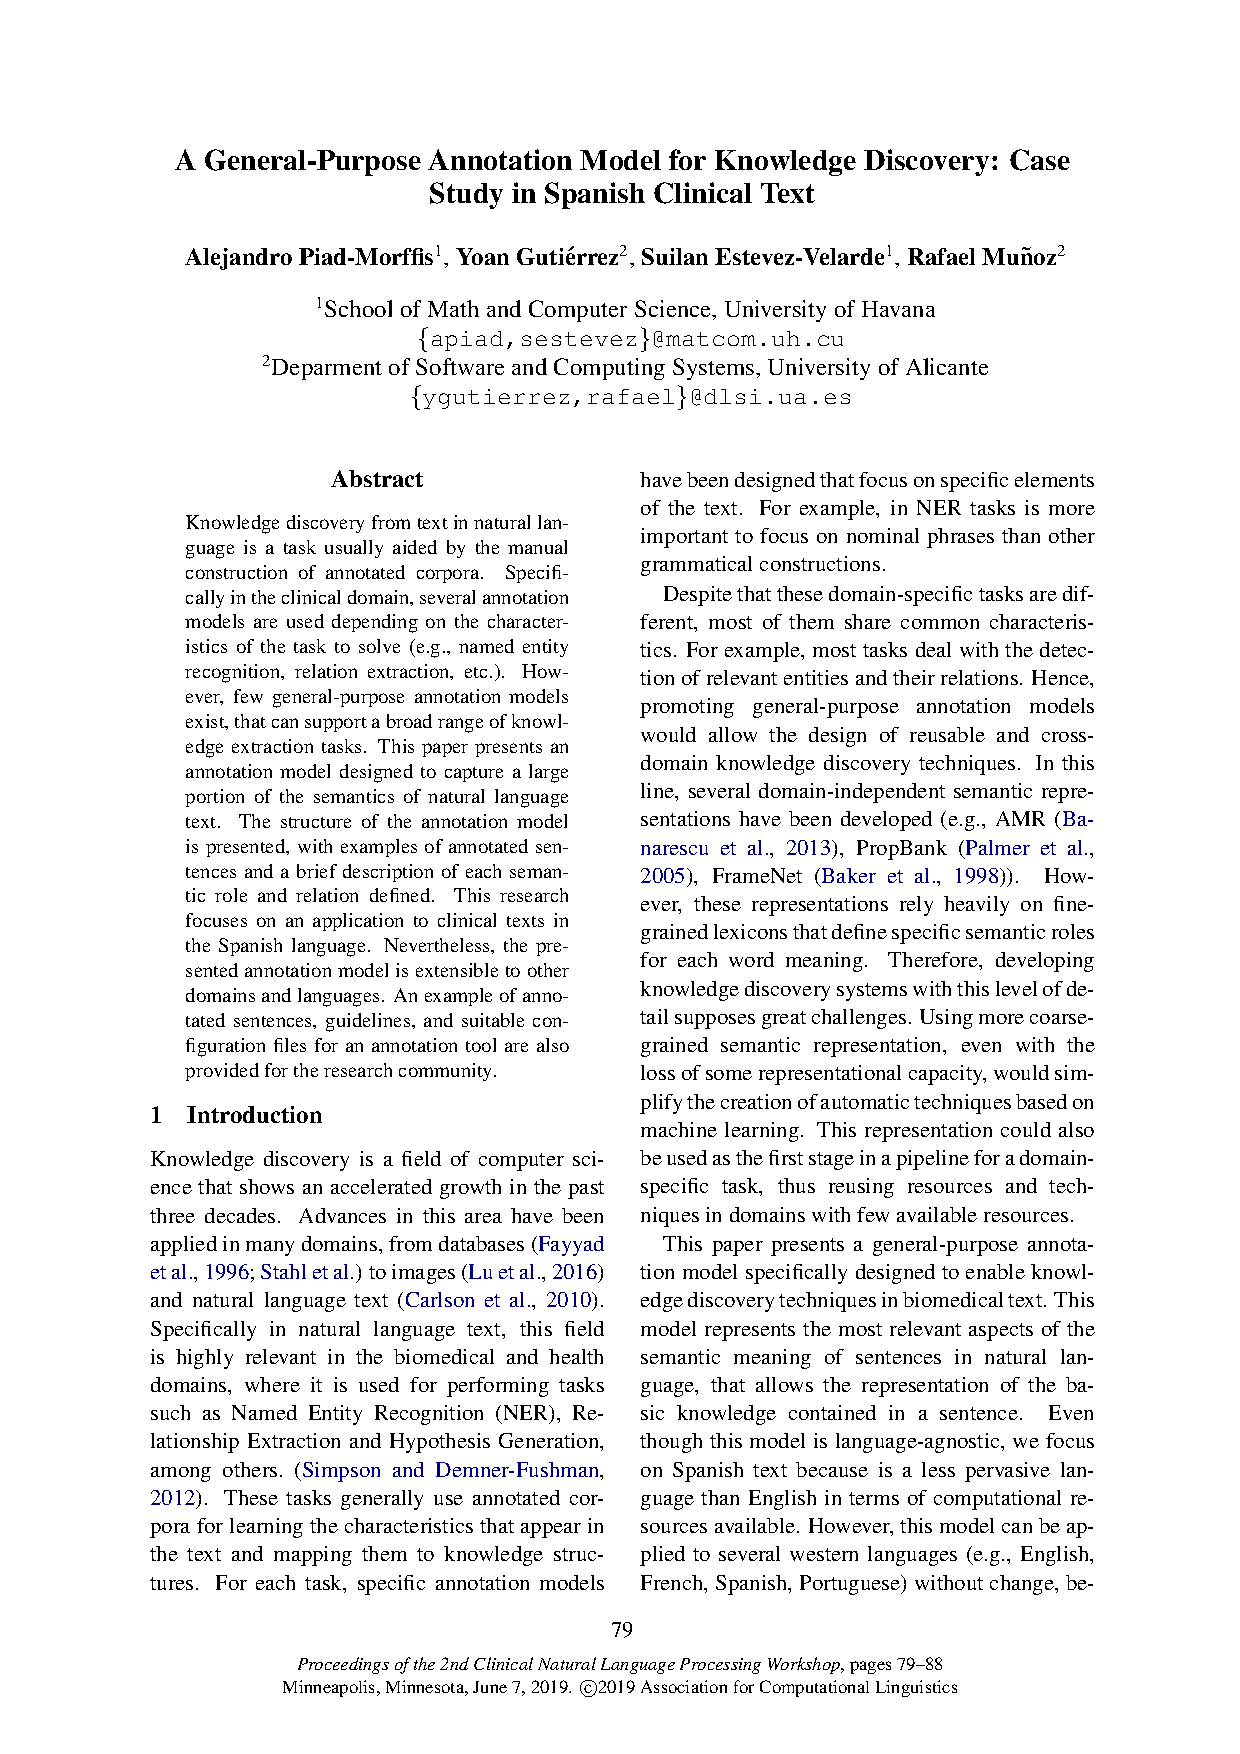
\includepdf[pages=1-, scale=0.9, offset=0 -0.75cm, pagecommand={\thispagestyle{fancy}}]{./Chapters/Papers/NAACL-Schema.pdf}

	
\chapter[Corpus eHealth-KD 2018: \textit{A corpus to support eHealth Knowledge Discovery technologies}]{Corpus eHealth-KD 2018}
\label{Chap:CorpusV1}

Ese capítulo presenta el artículo \textit{A corpus to support eHealth Knowledge Discovery technologies}.
Este artículo introduce y describe el corpus \textit{eHealth-KD 2018}. El corpus es una colección de $1173$ oraciones relacionadas con la salud en español anotadas manualmente con una estructura semántica general que captura la mayor parte del contenido, sin recurrir a etiquetas de dominio específico. La representación semántica se define e ilustra primero con oraciones de ejemplo del corpus. Se resume además el proceso de anotación y se proporcionan métricas relevantes del corpus. Finalmente, se presentan tres implementaciones computacionales, que son compatibles con los modelos de aprendizaje automático y fueron diseñadas para estimar la complejidad del aprendizaje de la semántica del corpus. El corpus resultante se utilizó como escenario de evaluación en TASS 2018 y se discuten los resultados obtenidos por los participantes. El corpus \textit{eHealth-KD} proporciona el primer paso en el diseño de un marco semántico de propósito general que se puede utilizar para extraer conocimiento de varios dominios.

\BlankLine
\noindent \textbf{Entrada bibliográfica:}\\
Piad-Morffis, A., Gutiérrez, Y., Muñoz, R. (2019). A corpus to support ehealth knowledge discovery technologies. \textit{Journal of Biomedical Informatics}, 94, 103172.

\BlankLine
\noindent \textbf{Disponible en:} \url{https://doi.org/10.1016/j.jbi.2019.103172}

    \includepdf[pages=1-, scale=1.05, offset=0 -0.75cm, pagecommand={\thispagestyle{fancy}}]{./Chapters/Papers/JBI-19.pdf}

    
\chapter[Ecosistema Computacional: \textit{A Computational Ecosystem to Support eHealth Knowledge Discovery Technologies in Spanish}]{Ecosistema Computacional}
\label{Chap:CorpusV2}

Este capítulo presenta el artículo \textit{A Computational Ecosystem to Support eHealth Knowledge Discovery Technologies in Spanish}. Este trabajo describe un ecosistema que facilita la investigación y el desarrollo en el descubrimiento del conocimiento en el dominio biomédico, específicamente en el idioma español. Con este fin, se desarrollan y comparten varios recursos con la comunidad de investigación, incluido un nuevo modelo de anotación semántica, un corpus anotado de 1.045 oraciones y recursos computacionales para construir y evaluar técnicas automáticas de descubrimiento de conocimiento. Además, se define una tarea de aprendizaje automático con criterios de evaluación objetivos, y se diseña un entorno de evaluación en línea, lo que permite a los investigadores interesados en esta tarea obtener resultados inmediatos y compararlos con el estado del arte. Como caso de estudio, se analizan los resultados de un evento competitivo basado en estos recursos y se brindan pautas para futuras investigaciones.

\BlankLine
\noindent \textbf{Entrada bibliográfica:}\\
Piad-Morffis, A., Gutiérrez, Y., Almeida-Cruz, Y., Muñoz, R. (2020). A computational ecosystem to support eHealth Knowledge Discovery technologies in Spanish. \textit{Journal of Biomedical Informatics}, 109, 103517.

\BlankLine
\noindent \textbf{Disponible en:} \url{https://doi.org/10.1016/j.jbi.2020.103517}

    \includepdf[pages=1-, scale=1.05, offset=0 -0.75cm, pagecommand={\thispagestyle{fancy}}]{./Chapters/Papers/JBI-20.pdf}

    \part{Artículos No Publicados}

    
\chapter[Anotación Asistida: \textit{Active Learning for Assisted Corpus Construction:A Case Study in Knowledge Discovery from Biomedical Text}]{Anotación Asistida}
\label{Chap:Annotation}

Este capítulo presenta el artículo \textit{Active Learning for Assisted Corpus Construction:A Case Study in Knowledge Discovery from Biomedical Text}.
Este artículo define un enfoque de aprendizaje activo que tiene como objetivo reducir el esfuerzo humano requerido durante la anotación de corpus en lenguaje natural, compuestos por entidades y relaciones semánticas. Nuestro enfoque ayuda a los anotadores humanos seleccionando inteligentemente las oraciones más informativas para anotar y pre-anotándolas con algunas entidades y relaciones semánticas. Se define una estrategia basada en la incertidumbre con un factor de densidad ponderado, utilizando métricas de similitud basadas en \textit{embeddings} de oraciones. Como caso de estudio, se evalúa este enfoque mediante simulación en el corpus \textit{eHealth-KD 2019} estimando la reducción potencial en el tiempo de anotación total. Los resultados experimentales sugieren que la estrategia de consulta reduce entre un $35\%$ y $40\%$ el número de oraciones que se deben anotar manualmente para desarrollar sistemas capaces de alcanzar un resultado objetivo de $F_1$,
mientras que la estrategia de pre-anotación produce una reducción adicional de $24\%$ en el tiempo total de anotación. En general, los experimentos preliminares sugieren que se podrían ahorrar hasta $60\%$ del tiempo de anotación produciendo corpus que tienen la misma utilidad para entrenar algoritmos de aprendizaje automático.

    \includepdf[pages=1-, scale=0.9, offset=0 -0.75cm, pagecommand={\thispagestyle{fancy}}]{./Chapters/Papers/EMNLP.pdf}

%%TC:endignore

    \part{Conclusiones y Recomendaciones}

    \pagestyle{fancyNormalChapterStyle}	% - Fixing style for the regular chapters

    %   <Conclusions>   %
    \chapter{Conclusiones}\label{Chap:Conclusions}
\markboth{\MakeUppercase{Conclusiones}}{}

El volumen de información que se publica cada día es una fuente de conocimiento relevante de gran utilidad para la comunidad científica. A partir del análisis de múltiples fuentes es posible encontrar conexiones que permitan potencialmente descubrir nuevo conocimiento que se encuentra disperso en las redes.
A pesar de esto, el alto número de fuentes a revisar es imposible de procesar por humanos, lo que dificulta este proceso de descubrimiento de conocimiento.
En este contexto cobra especial relevancia el desarrollo de técnicas automáticas para la extracción y descubrimiento de este conocimiento.

El dominio de la salud es uno de los que más puede beneficiarse del descubrimiento automático de conocimiento, debido a la velocidad y el volumen con el que se publican nuevos resultados. La reciente pandemia de COVID-19 es solo un ejemplo más de la necesidad de conectar de forma automática los hechos y resultados publicados a diario. Para construir sistemas computacionales capaces de realizar esta tarea, es necesario no solo la creación de recursos lingüísticos que sirvan para los modelos de aprendizaje automático, sino también la creación de una infraestructura que permita a los investigadores evaluar sus sistemas de forma efectiva y compararlos con el estado del arte.

Esta investigación presenta el diseño y la construcción de un ecosistema para el desarrollo de tecnologías de descubrimiento de conocimiento, enfocado en el dominio de la salud y el idioma español.
Este ecosistema incluye recursos lingüísticos, herramientas computacionales y una metodología para la evaluación de nuevos enfoques.

Con el objetivo de representar de forma computacionalmente manejable el lenguaje natural, se definió un modelo de anotación para capturar el contenido semántico más relevante de una oración, basado en una estructura Sujeto-Acción-Objetivo y relaciones semánticas adicionales.
El modelo no incluye entidades o relaciones de dominio específico para ser lo más general posible. Este modelo está diseñado para ser suficientemente expresivo pero que aún así sea factible tanto su anotación por expertos humanos con un alto grado de acuerdo entre diferentes anotadores como la aplicación de técnicas de aprendizaje automático.

Basado en este esquema de anotación, se anotaron manualmente a lo largo de la investigación cuatro versiones de un corpus con un total de $41,163$ elementos semánticos repartidos en $3,068$ oraciones, tomando como base información en el dominio de salud en idioma español. A pesar del enfoque en el dominio de la salud, a modo de caso de estudio se incluyen $300$ oraciones en un dominio alternativo (reportajes periodísticos), $200$ oraciones en idioma inglés, que demuestran la capacidad de generalización del esquema de anotación. Los cuatro versiones de un corpus fueron anotados por equipos compuestos por anotadores expertos y no expertos, siguiendo un protocolo que garantizó un alto grado de acuerdo en los elementos anotados.
El propósito de estos recursos lingüísticos es permitir la creación de sistemas de descubrimiento de conocimiento a partir del uso de técnicas de aprendizaje automático.
Con este propósito, se ha organizado una campaña de evaluación, \textit{eHealth-KD challenge}, de la que se han producido cuatro ediciones consecutivas. En total han participado un total de $33$ equipos de investigadores de diferentes nacionalidades con múltiples estrategias, principalmente enfocadas en arquitecturas de aprendizaje profundo. Para permitir una comparación entre diferentes sistemas, se diseñó un escenario que consiste de dos subtareas fundamentales, y se definieron un conjunto de métricas para su evaluación.
Los resultados obtenidos en las cuatro ediciones de esta campaña demuestran que el reto de descubrir conocimiento automáticamente en lenguaje natural es un problema aún abierto pero se ha producido una mejora considerable en la efectividad de los sistemas presentados de una edición a la siguiente, fomentado por el reciente desarrollo de nuevas arquitecturas de aprendizaje profundo para el procesamiento de lenguaje natural.

Más allá de las ediciones de la campaña \textit{eHealth-KD}, esta investigación se propuso construir un ecosistema de evaluación continua que pueda ser utilizado de forma independiente por cualquier investigador para evaluar nuevos enfoques y compararse con el estado del arte.
Este ecosistema se pone a disposición de la comunidad científica, que consiste una infraestructura y un conjunto de herramientas (incluyendo implementaciones básicas con las que compararse), un entorno de evaluación continua en la nube, y estadísticas actualizadas sobre el estado del arte de la tarea \textit{eHealth-KD}.
Todos estos recursos, incluyendo los corpus anotados y las herramientas computacionales están publicados bajo licencias de código abiertas y disponibles para su uso en línea\footnote{\url{https://ehealthkd.github.io}}.

Finalmente, a partir de las experiencias acumuladas durante el proceso de anotación, se implementó un sistema de anotación asistida que permite reducir considerablemente el costo manual de producir nuevos recursos lingüísticos en esta área.
Este sistema utiliza técnicas de aprendizaje automático para seleccionar las oraciones más útiles a anotar, y garantizar un balance de los datos en un corpus con el menor esfuerzo posible por parte de los anotadores humanos.
Esta herramienta está basada en componentes de código abierto y se encuentra disponible para el uso de la comunidad científica\footnote{\url{https://github.com/knowledge-learning/assisted-annotation}}.

Todos los resultados presentados en esta Tesis son parte de una línea de investigación activa para aprovechar la semántica de propósito general y las tecnologías basadas en el conocimiento junto con las nuevas arquitecturas de aprendizaje profundo en la construcción de tecnologías automáticas de descubrimiento de conocimiento.
Como parte de esta línea, se continúa trabajando en la expansión de los recursos lingüísticos creados y en la organización de campañas de evaluación para fomentar la investigación en esta temática en la comunidad, así como en el desarrollo de nuevas herramientas computacionales basadas en técnicas de aprendizaje automático para el descubrimiento de conocimiento a partir de lenguaje natural.

\section{Publicaciones}
\label{Chap:Conclusions-Publications}

Los resultados de investigación parciales que conforman esta tesis se han publicado anteriormente en diversos artículos. A continuación se listan aquellas publicaciones relacionadas con esta investigación en las que ha participado el autor:

\begin{itemize}
    \item Overview of TASS 2018: Opinions, health and emotions~\cite{tamartinez2018overview}
    \item Overview of the eHealth Knowledge Discovery Challenge at IberLEF 2019~\cite{tapiad2019overview}
    \item Overview of the eHealth Knowledge Discovery Challenge at IberLEF 2020~\cite{piad2020overview}
    \item Overview of the eHealth Knowledge Discovery Challenge at IberLEF 2021~\cite{piad2021overview}
    \item A general-purpose annotation model for knowledge discovery: Case study in Spanish clinical text~\cite{tapiad2019general}
    \item A corpus to support eHealth Knowledge Discovery technologies~\cite{piad2019corpus}
    \item A Computational Ecosystem to Support eHealth Knowledge Discovery Technologies in Spanish~\cite{piad2020computational}
    \item Gathering object interactions as semantic knowledge~\cite{taestevez2018gathering}
    \item TASS 2018: The strength of deep learning in language understanding tasks~\cite{tass}
    \item A Neural Network Component for Knowledge-Based Semantic Representations of Text~\cite{tapiad2019neural}
    \item Analysis of eHealth knowledge discovery systems in the TASS 2018 workshop~\cite{taalejandro2019analysis}
    \item Active Learning for Assisted Corpus Construction:A Case Study in Knowledge Discovery from Biomedical Text~\cite{canizares2021active}
    \item Knowledge Discovery in COVID-19 Research Literature~\cite{estevanell2021knowledge}
\end{itemize}

Adicionalmente, se listan a continuación las ediciones del evento \textit{eHealth Knowledge Discovery} organizadas como parte del marco de evaluación de esta investigación:

\begin{itemize}
    \item eHealth KD 2018 como Workshop en el evento TASS 2018\\ \url{http://www.sepln.org/workshops/tass/2018/task-3}
    \item eHealth KD 2019 como Workshop en el evento IBERLEF 2019\\ \url{https://knowledge-learning.github.io/ehealthkd-2019}
    \item eHealth KD 2020 como Workshop en el evento IBERLEF 2020\\ \url{https://knowledge-learning.github.io/ehealthkd-2020}
    \item eHealth KD 2021 como Workshop en el evento IBERLEF 2021\\ \url{https://ehealthkd.github.io/2021}
\end{itemize}


    \chapter{Trabajo Futuro}\label{Chap:FutureWork}
\markboth{\MakeUppercase{Trabajo Futuro}}{}

La investigación desarrollada en esta tesis puede ser continuada desde múltiples perspectivas.
En primer lugar, los modelos teóricos de representación del conocimiento diseñados así como los algoritmos presentados, pueden ser mejorados y adaptados a nuevos escenarios.
Por otro lado, el ecosistema diseñado permite continuar con la organización de eventos competitivos en diferentes tareas y dominios para incentivar el desarrollo de nuevas técnicas de descubrimiento de conocimiento.
En este capítulo se presentan las ideas que consideramos más relevantes y que pueden proveer un mayor aporte a los resultados y aplicaciones futuras de esta investigación.

Desde la arista de desarrollo y creación de corpus, una de las líneas de investigación más claras es la anotación de nuevos recursos lingüísticos en otros dominios e idiomas. 
Entre los dominios más interesantes a analizar se encuentran los artículos científicos, las noticias y los artículos enciclopédicos. Estas son fuentes de información factual que presentan diferentes características sintácticas pero que potencialmente pueden ser capturadas con las mismas estructuras semánticas definidas en esta investigación.
Anotar nuevos dominios permitiría también ampliar el \textit{eHealth-KD} a una audiencia mayor, por ejemplo, los investigadores interesados en el fenómeno de las noticias falsas.
Además, esto abre las puertas a la definición de tareas multi-dominio, donde los mismos sistemas sean evaluados en corpus de dominios diferentes a los que fueron entrenados, requiriendo el desarrollo de técnicas de transferencia de aprendizaje automático.

En la dirección de modernizar la tarea \textit{eHealth-KD} hay dos escenarios nuevos interesantes de explorar.
En primer lugar, adicionar el problema de reconocimiento de los atributos, que actualmente son anotados en el corpus pero no evaluados en la tarea. Este escenario ya introduce algunos problemas computacionales interesantes, por ejemplo, la identificación de la negación y su ámbito.
Con vistas a avanzar hacia una representación semántica de más alto nivel, el otro escenario de interés consiste en la normalización de las entidades extraídas en función de bases de datos estructuradas, por ejemplo, Wikidata.
Estas adiciones complejizan la tarea \textit{eHealth-KD}, pero como mismo se separan la extracción de entidades y relaciones en diferentes subtareas, se pueden definir subtareas específicas para estos problemas permitiendo que investigadores especializados en un área participen en aquellos problemas de su interés.

El esquema de anotación propuesto en esta investigación ha demostrado ser capaz de capturar una porción significativa de la semántica del lenguaje natural. Sin embargo, aún mantiene algunas inconsistencias y ambigüedades que pueden ser mejoradas con pocas modificaciones. 
Una de las principales fuentes de ambigüedad identificada es la similitud entre los roles de \texttt{Predicate} y la relación \texttt{in-context}. Es posible que una de estas variantes sea redundante, o que deba definirse de manera más clara la diferencia entre ambos patrones de anotación.
La adición más importante al esquema de anotación consistiría en un nuevo tipo de relación semántica que permita denotar el propósito de una acción o evento.

Finalmente, la estrategia de aprendizaje activo desarrollada en la investigación brinda una solución prometedora al problema del costo de la anotación manual, pero solo ha sido evaluada en escenarios simulados.
La propuesta más relevante en este sentido consiste en aplicar esta estrategia para la anotación de los recursos lingüísticos de la próxima edición del \textit{eHealth-KD}.
Para esto es necesario adaptar la propuesta a un escenario con múltiples anotadores por cada oración.
En este escenario, el propio desacuerdo entre los anotadores introduce una nueva fuente de incertidumbre que puede ser utilizada para optimizar el proceso de anotación.

Las ideas sugeridas en este capítulo son solo algunas de las posibilidades más claras para continuar el desarrollo de las técnicas y recursos propuestos en esta tesis. El trabajo desarrollado forma parte de una línea de investigación activa. Estas y otras ideas serán tenidas en cuenta para estimular aún más el desarrollo de tecnologías de descubrimiento de conocimiento, siempre desde la perspectiva de aprovechar el esfuerzo humano y los recursos computacionales en estrecha colaboración. Visualizamos un futuro donde los seres humanos y las computadoras trabajen juntos en la solución de los problemas más apremiantes, cada uno poniendo sus mejores habilidades al servicio de las futuras generaciones.


	%	<Conclusions-FutureWork>	%
	%\include{./Chapters/Conclusions-FutureWork/Conclusions-FutureWork}

	%	<Part : Appendix>	%
% 	\appendix

% 	\pagestyle{fancyAppendixStyle}	% - Fixing style for the appendices

% 	%   <Annotation Guidelines> %
% 	\include{./Chapters/Annotation-Guidelines/Annotation-Guidelines}

% 	%	<Summary-Spanish>	%
% 	\include{./Chapters/Summary-Spanish/Summary-Spanish}

	\backmatter

	%	<Bibliography>	%
	\pagestyle{fancyUnnumberedSectionsStyle}	% - Fixing style for the regular chapters

    \bibliographystyle{unsrtnat}
	\bibliography{./Bibliography/Bibliography}


	%	<Nomenclature>	% (omitted for the moment)
	%I want $\beta$\nomenclature{$\beta$}{The second letter of the greek alphabet} to be listed after $\alpha$\nomenclature{$\alpha$}{The first letter of the greek alphabet} % Only to try...

	%\printnomenclature

\end{document}
